% !TEX root = base.tex 

\chapter{Background}
\label{ch:background}

\chintro{This chapter provides background information for the research presented in this document. The basics of semiconductor photochemistry are presented, as well as background on the effect of p-n junctions, ferroelectric polarization, and polar surfaces on photochemistry. The crystallography and relevant properties of the materials utilized in this document are also included.}

\section{Photochemistry on Semiconductor Surfaces}
\label{sec:background.semiconductorphotochem}

When a semiconductor is illuminated by a photon with energy larger than the semiconductor's band gap, the photon can be absorbed by the semiconductor.\cite{Morrison:1980va} In this process, an electron is excited to the conduction band, leaving behind a hole in the valence band. If the electron-hole pair is generated near the surface, or is driven to the surface by an electric field, it can participate in surface chemical reactions. The process is illustrated schematically in \figureref{photochemsteps}.

\begin{figure}
	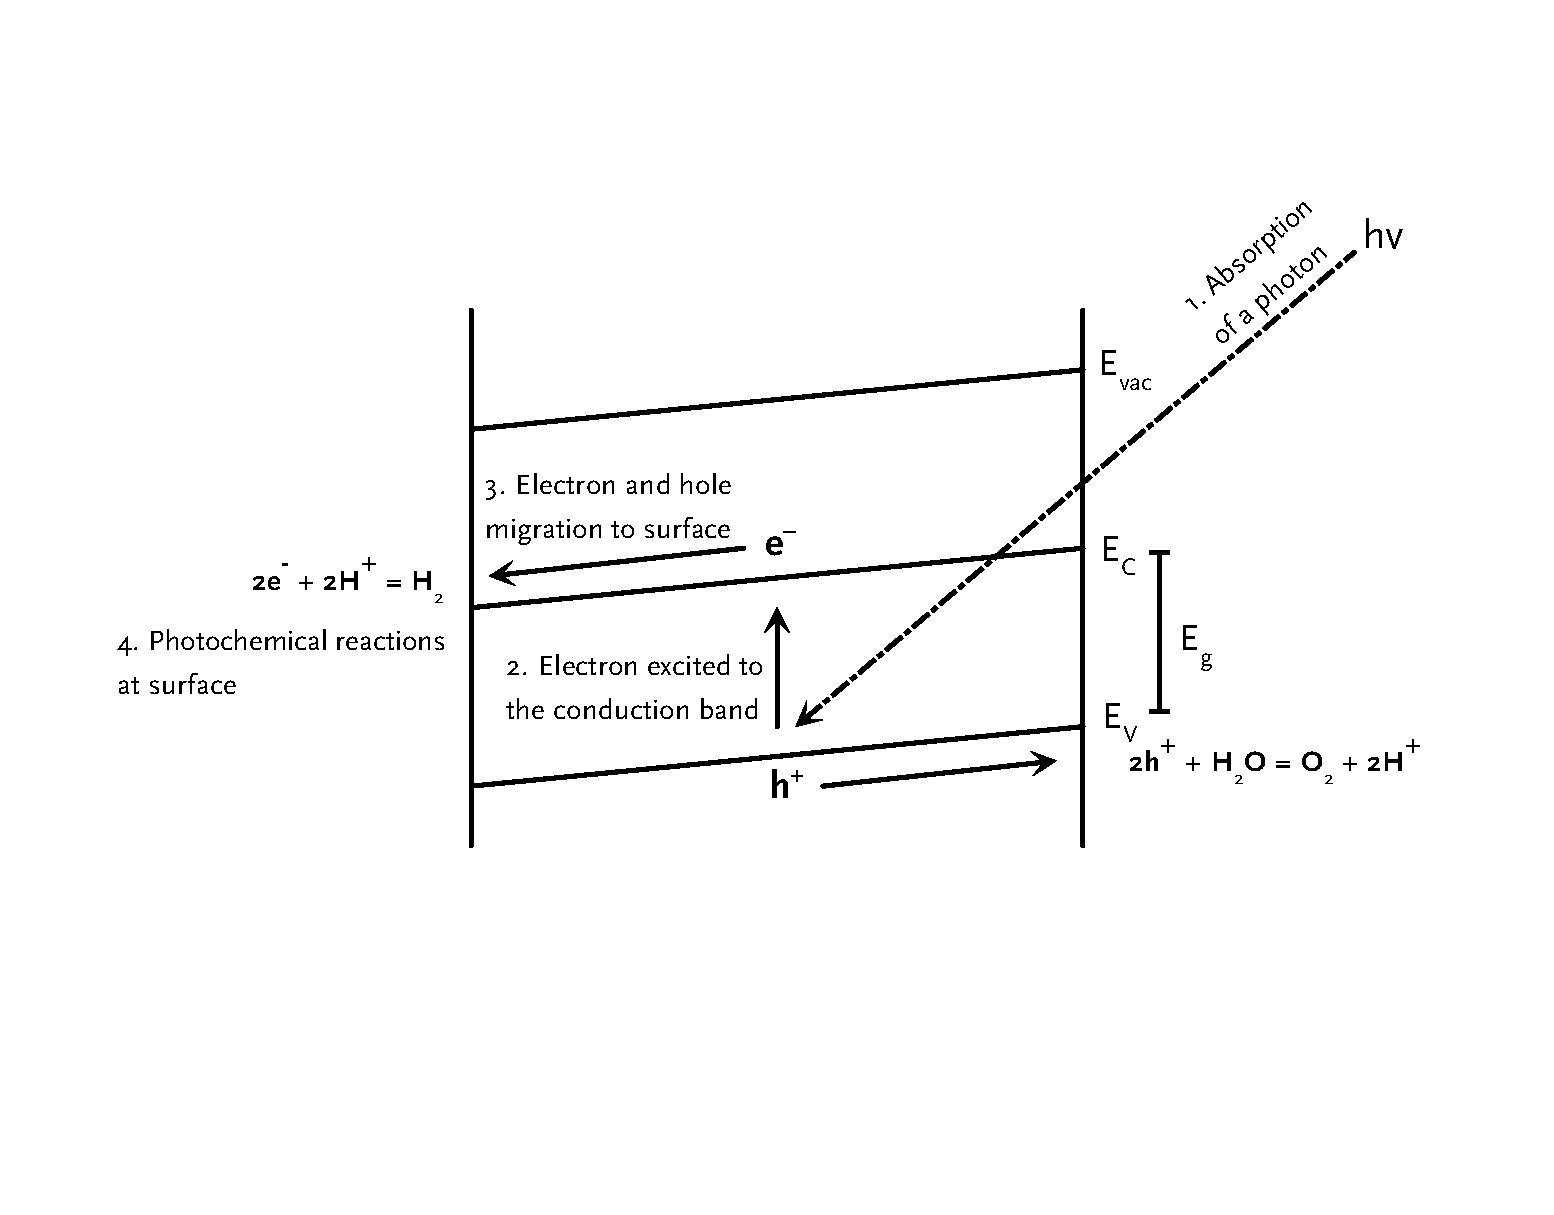
\includegraphics[width=\textwidth]{photochemsteps.pdf}
	\caption[Simplified schematic of the water photolysis process]{%
		Simplified schematic of the water photolysis process. A photon 
		with an energy larger than the band gap is absorbed, exciting 
		an electron from the conduction band to the valence band. The 
		electron and hole are driven to the opposite surfaces by an electric field, 
		represented here by sloped bands. At the surface, the charge 
		carriers take part in photochemical reactions.}
	\label{fig:photochemsteps}
\end{figure}

For water splitting (water photolysis),\cite{memming2001semiconductor} the electrons and holes are used to drive the following reactions:
\begin{gather}
	\ce{2H+ + 2e^{-} -> H2_{(g)}} \hspace{1.5em} \text{(Reduction)}\\
	\ce{H2O + 2h+ -> 1/2O2_{(g)} + 2H+} \hspace{1.5em} \text{(Oxidation).}
\end{gather}
Only electrons and holes with appropriate electrochemical potentials can promote these reactions. The conduction band edge of the semiconductor must lie above the potential of the reduction reaction and the valence band edge must be below the potential for oxidation. An effective photocatalyst has a band gap that is both large enough to promote both reactions and is properly located in relation to the potential of each reaction. For water splitting, the hydrogen and oxygen half reactions are located at 0~V and 1.23~V respectively,\cite{noauthororeditor2007handbook} on the hydrogen scale. This requirement on the band gap and energy levels of potential photolysis catalysts is non-trivial. \figureref{morrisonarray} shows an array of the valence and conduction band energies of potential materials for water photolysis.\cite{Morrison:1980va} Only materials with electron and valence band energies in the white area of the array satisfy both requirements on the position of the energy levels of the semiconductor. Significant research efforts\cite{Osterloh:2008fp} are invested in the discovery and synthesis of new materials that satisfy the necessary energy requirements for water photolysis. 

\begin{figure}
	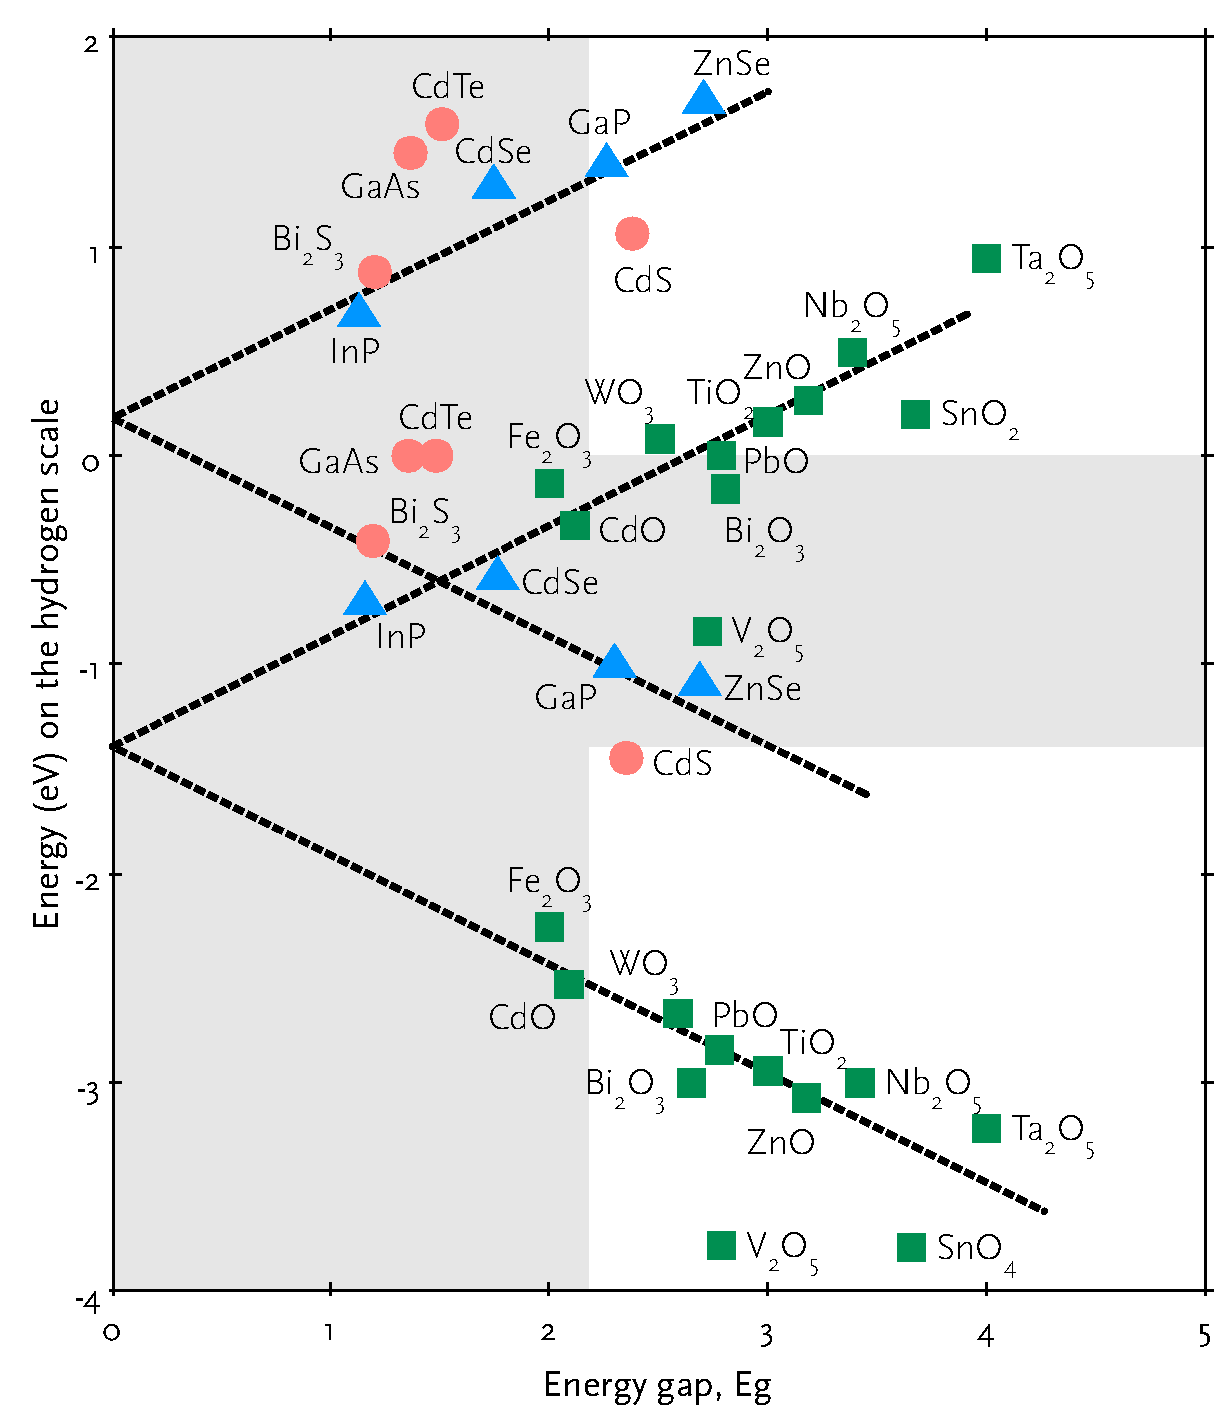
\includegraphics[width=0.95\textwidth]{morrisonarray.pdf}
	\caption[Array of band positions for semiconductors]{%
		Array of band positions for traditional and oxide semiconductors. 
		The area shaded in blue less than \texttildelow2.1~eV represents 
		materials unsuitable for water splitting, as the band gap is not 
		large enough to drive water splitting when overpotentials are 
		considered. The shaded blue area between -1.23~eV and 0 eV on the 
		hydrogen scale represents the position on the energy scale that 
		must be straddled by the band positions. The valence band must be 
		below -1.23 eV and the conduction band must lie above 0~eV.\cite{Morrison:1980va}}
	\label{fig:morrisonarray}
\end{figure}


\subsection{Photolysis and the Solar Spectrum}
\label{subsec:background.solarspectrum}


Before water photolysis can serve as a viable method of hydrogen production, systems must be made less expensive and more efficient. Major limitations on the efficiency of water photolysis are the separation of photogenerated charge carriers in the material and the utilization of a wider portion of the solar spectrum. After a photon is absorbed in a semiconductor and an electron is excited to the valence band, the electron or hole must reach the surface before recombining. Recombination is the process by which a photogenerated charge carrier combines with an oppositely charged carrier. Recombined electron-hole pairs represent lost efficiency, as the recombined electron no longer contains the necessary energy to drive photochemical reactions. 



\begin{figure}
	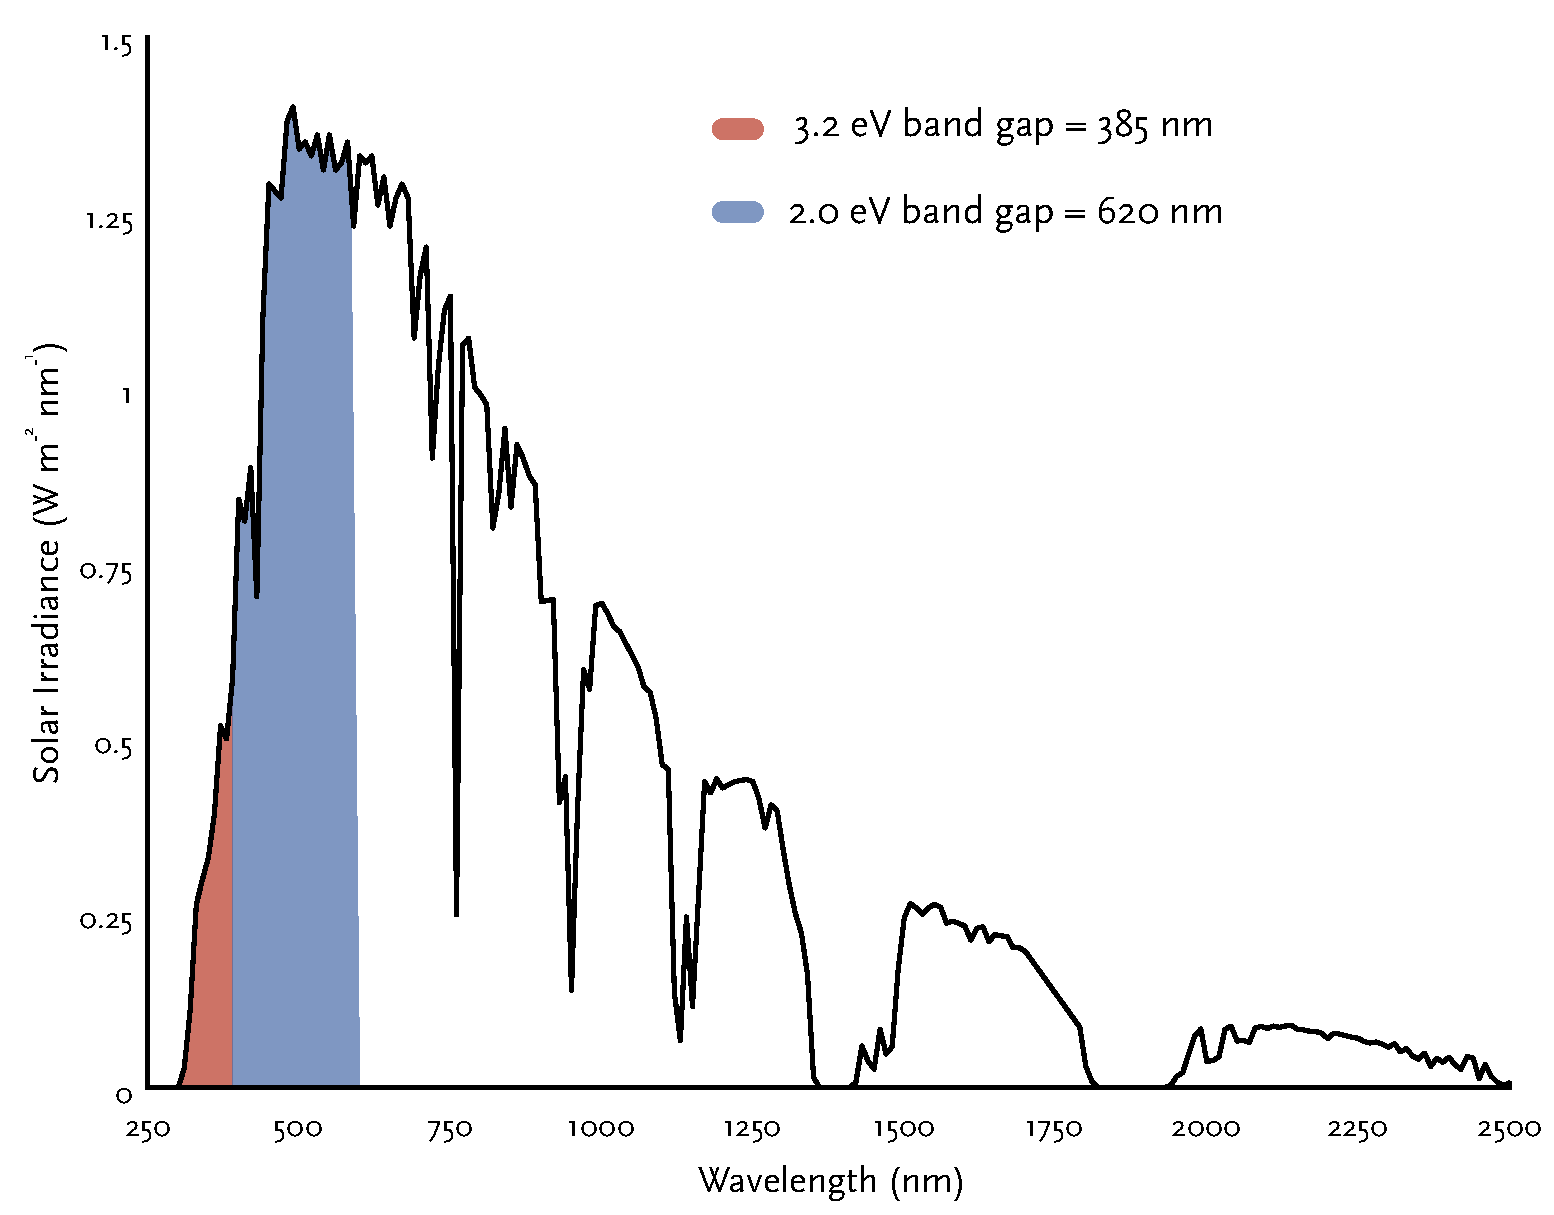
\includegraphics[width=\textwidth]{solarspectrum.pdf}
	\caption[Solar irradiance at the earth 's surface]{%
		Solar irradiance at the earth 's surface as a function of 
		wavelength. The shaded regions represent the portion of the 
		solar spectrum that can be utilized by a semiconductor with a 
		3.2~eV band gap (red) and a 2.0 eV band gap (blue).\cite{Anonymous:jk}}
	\label{fig:solarspectrum}
\end{figure}

The solar spectrum is shown in \figureref{solarspectrum}. The majority of the light reaching the earth's surface lies in the visible range of the electromagnetic spectrum, corresponding to photon energies of 1.6~eV to 3~eV. Titanium dioxide, \ce{TiO2}, one of the most studied photocatalysts, has a band gap of 3.2~eV. This value is well in to the ultraviolet portion of the solar spectrum. Only 2\% of the light reaching the earth's surface is of sufficient energy to excite an electron in \ce{TiO2}. This means that for \ce{TiO2}, 98\% of solar radiation is unavailable for use in water splitting. Moving to materials with a smaller band gap that can utilize light in the visual portion of the spectrum greatly increases the percent utilization of the solar spectrum. A shift to a material with a band gap of 2.0~eV, corresponding to orange light, represents an increased maximum absorption efficiency of using 34\% of the solar spectrum. It should be noted that the absorption efficiency is always greater than the overall efficiency. Each absorbed photon is used to perform 1.23~eV of work, regardless of the energy of the photon. Any excess energy of the photon over the minimum for water splitting represents lost efficiency of the overall system. This goal of shifting to materials with smaller band gaps adds additional complexity to the selection of photolysis catalysts when viewed in connection with \figureref{morrisonarray}. Smaller band gaps are desirable to make use of a wider portion of the solar spectrum, but the band edges must be located correctly in relation to the levels for the reactions of water splitting.

\subsection{Photolysis Systems}
\label{subsec:background.systems}

Currently, research has concentrated on two systems for photolytic hydrogen evolution. The photoelectrochemical cell has shown promising efficiencies,\cite{Fujishima:1972hc,User:2001tg} however it is too expensive for large scale hydrogen production. Particulate photocatalysts have the potential to be much less expensive than photoelectrochemical cells, however their efficiencies are much lower. \cite{Kaneko:2002vh} Because the electrodes in the particle catalysts are not physically separated as in the photoelectrochemical cell, charge carrier recombination limits the efficiency of the catalyst. Much of the work on particulate photocatalysts centers on creating physical separation of the anode (oxidation sites) and cathode (reduction sites).\cite{Kitano:2008io,Kudo:2008fk} Schematics of the photoelectrochemical cell and particulate photocatalyst are depicted in \figureref{pecparticle}.

\begin{figure}
	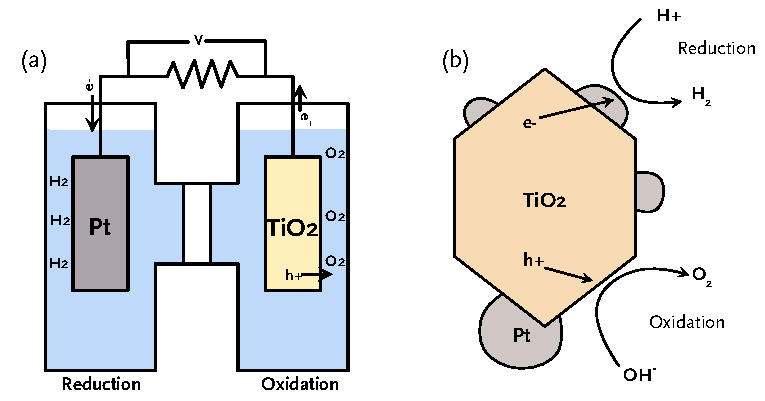
\includegraphics[width=\textwidth]{pecparticle.pdf}
	\caption[Photoelectrochemical and particulate cells]{%
		(a) Photoelectrochemical cell. When light shines on the TiO2 
		electrode, an electron-hole pair is generated. The electron 
		travels through an external `circuit to the platinum electrode, 
		where it generates hydrogen. The hole generates oxygen at the 
		surface of the \ce{TiO2} electrode. (b) A particulate cell. 
		In this case, oxidation and reduction occur on the same particle.}
	\label{fig:pecparticle}
\end{figure}

In the photoelectrochemical cell depicted in \figureref{pecparticle}(a), the \ce{TiO2} electrode is illuminated, generating electrons and holes. The holes participate in oxidation at the \ce{TiO2} electrode, generating oxygen. The electrons travel through an external circuit to a platinum electrode separated by a salt bridge. At the platinum electrode, the electrons reduce hydrogen ions to form hydrogen gas. The particulate catalyst in \figureref{pecparticle}(b) represents a short-circuited version of the photoelectrochemical cell. Electrons and holes are generated in the \ce{TiO2} under illumination. Holes oxidize water at the surface of the \ce{TiO2} surface, while electrons travel to hydrogen particles on the surface, where they participate in reduction.


\subsection{Length Scales in Photochemistry}
\label{subsec:background.lengthscales} %% In response to overview feedback point 7b

\begin{figure}
\begin{center}
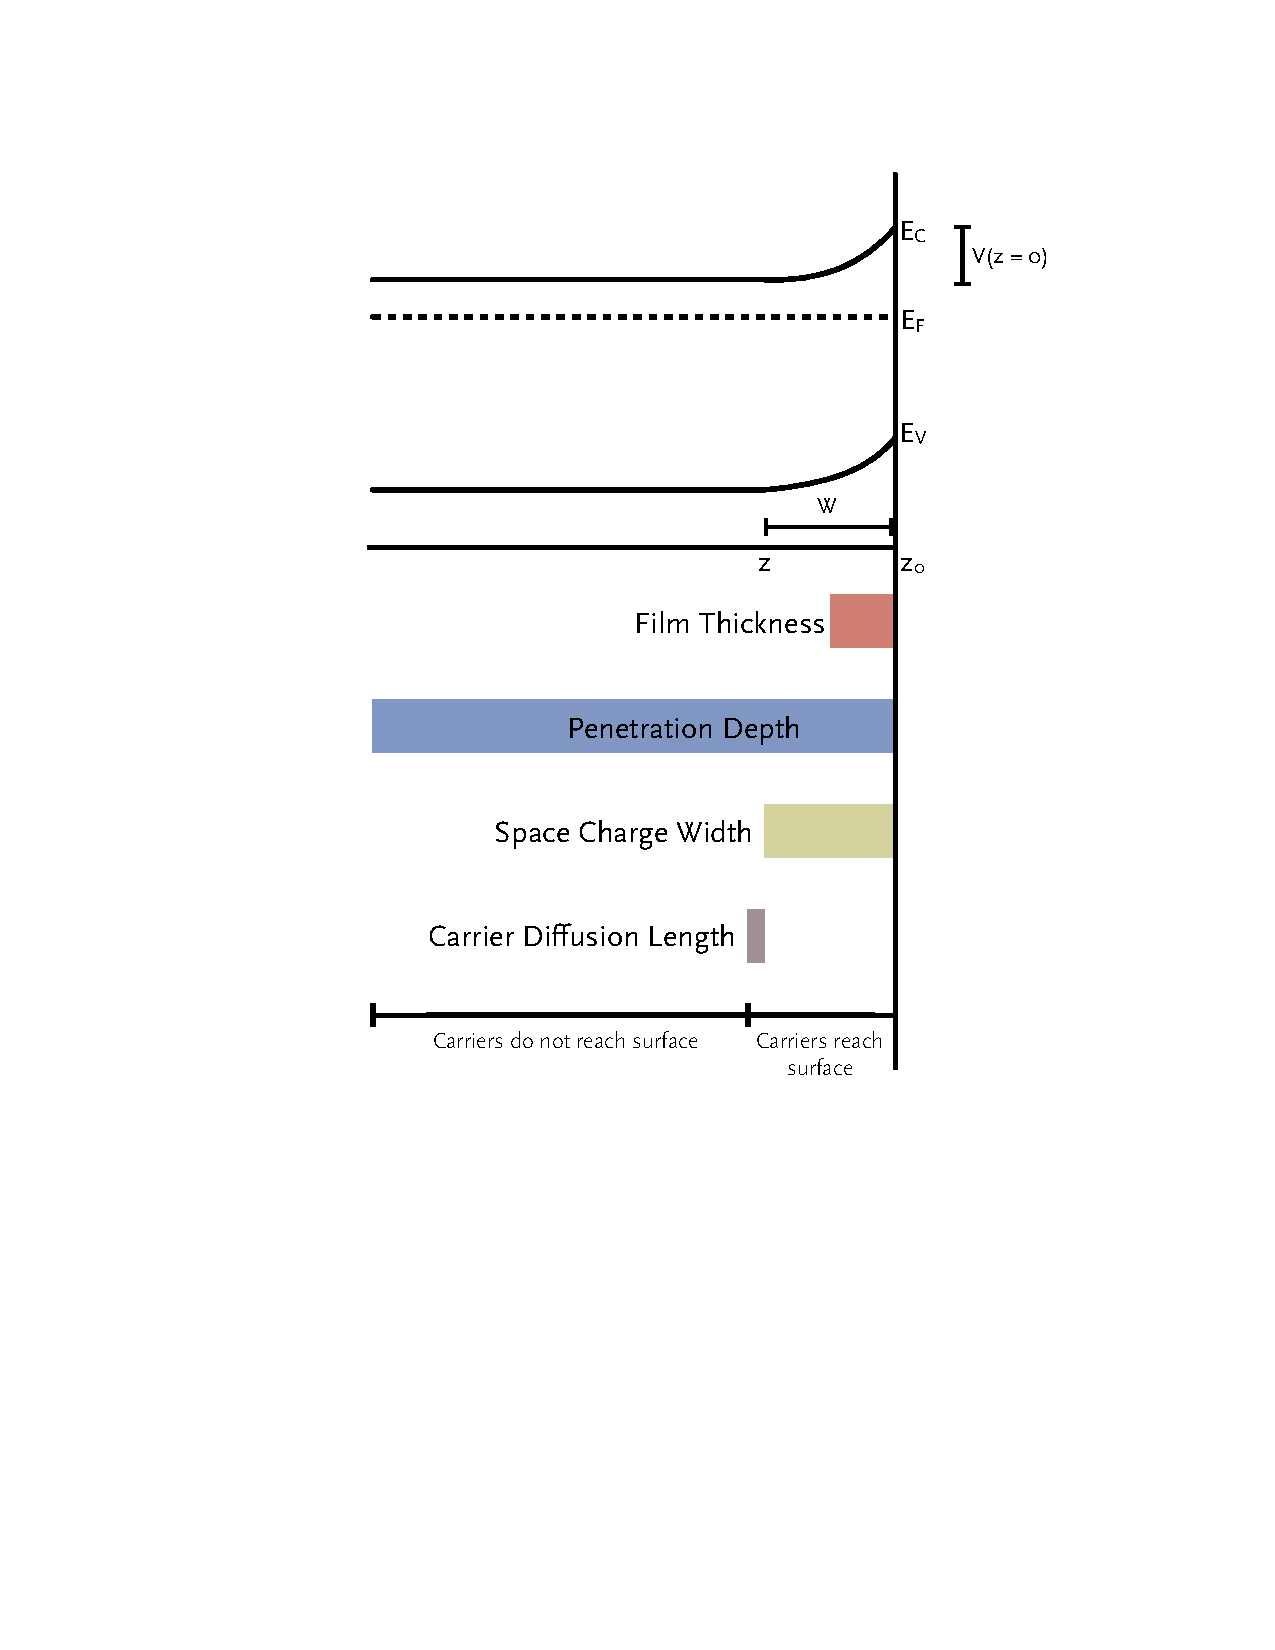
\includegraphics[width=0.6\textwidth]{lengthscales.pdf}
\caption[Band bending at semiconductor surface]{%
	Schematic energy level diagram showing band bending at a semiconductor 
	surface, along with a depiction of typical length scales relevant to 
	semiconductor photochemistry.}
\label{fig:lengthscales}
\end{center}
\end{figure}
%\sidefigure[Band bending at semiconductor surface]{%
%	Schematic energy level diagram showing band bending at a semiconductor 
%	surface, along with a depiction of typical length scales relevant to 
%	semiconductor photochemistry.
%	\label{fig:lengthscales}
%	}{%
%	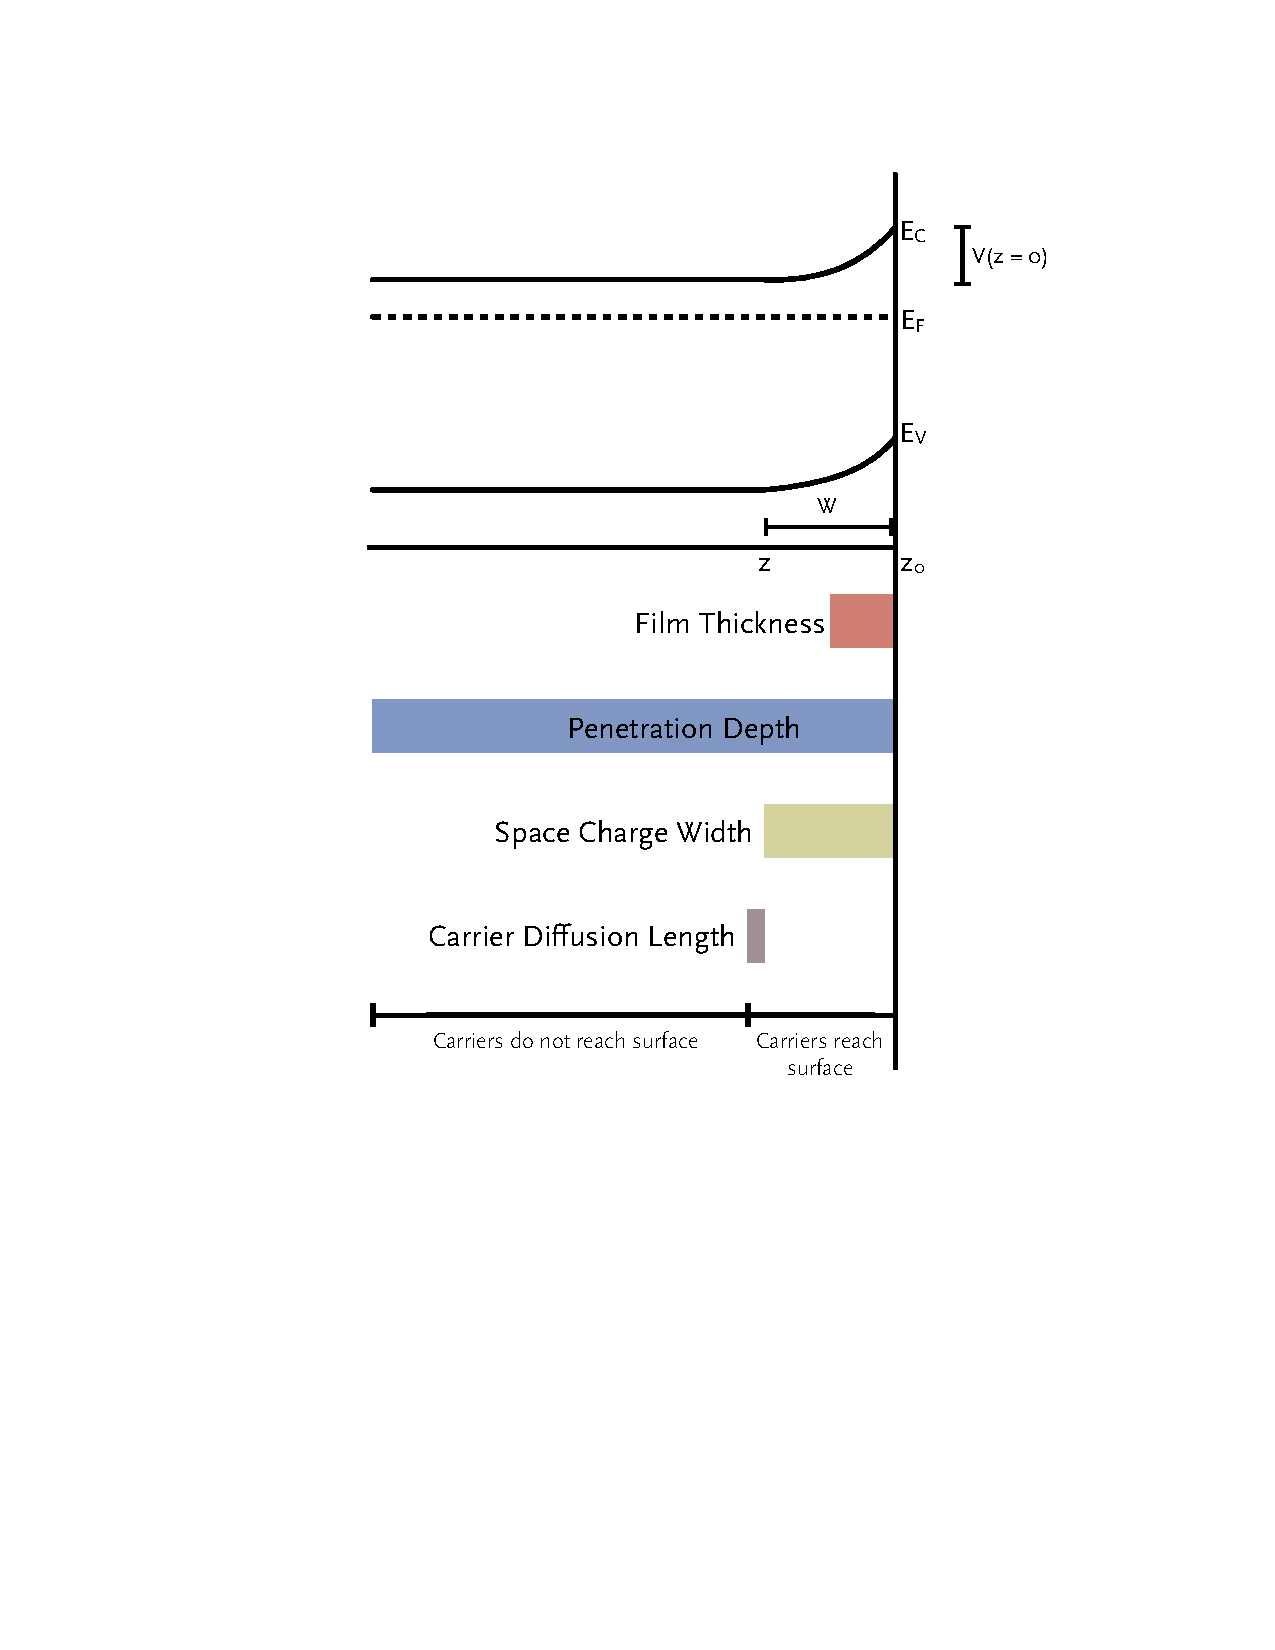
\includegraphics[width=\marginparwidth]{lengthscales.pdf}
%}{0}

A number of competing characteristic length scales play an important role in semiconductor photochemistry. The ideal photolysis catalyst must optimize these characteristic lengths to achieve high efficiencies. The relevant lengths are labelled and compared in \figureref{lengthscales}. Each is discussed in the following section, including its importance to semiconductor photochemistry, relative magnitude, and relation to other relevant parameters.

The penetration depth of light into the semiconductor is the first important length to consider. Not all light is absorbed directly at the surface of the semiconductor. Instead, light penetrates into the semiconductor, its intensity decreasing as it travels further into the crystal and photons are absorbed. The penetration into the crystal is a function of the material's absorption coefficient, which itself is a function of light wavelength. The Beer-Lambert law (Eq. \ref{eq:beerlambert}) describes how the intensity of incident light decays within a material, where $z$ is the depth within the material and $\alpha$ is the absorption coefficient. The penetration depth is defined as the depth within the material where the ratio of intensity to incident intensity is reduced to  $\frac{1}{e}$ (Eq. \ref{eq:definepenetrationdepth}). This point occurs at $\frac{1}{\alpha}$ (Eq. \ref{eq:oneoveralpha}).

\begin{gather}
	\label{eq:beerlambert}
	I(z)=I_{0}e^{-\alpha z},\\
	\label{eq:definepenetrationdepth}
	\delta_{p} \equiv \frac{I(z)}{I_{0}}=\frac{1}{e},\\
	\label{eq:oneoveralpha}
	\delta_{p} = \frac{1}{\alpha}.
\end{gather}

For hematite under illumination by a \SI{470}{\nano\meter} blue LED (the material and light source used in the majority of experiments presented in this document), the penetration depth is \texttildelow\SI{450}{\nano\meter}.\cite{Marusak:1980gc} The majority light absorption occurs within this length, and consequently the majority of electron-hole pairs are generated within this length.

Once an electron-hole pair is generated through the absorption of a photon, it must reach the surface to participate in a chemical reaction. If the electron-hole pair is generated within an electric field,  that field will cause the electron and hole to move in opposite directions, causing one of the carriers to reach the surface. In the heterostructures used for experiments in this document, electric fields arise from built in sources. Details of these sources are presented in \S\ref{sec:background.charged}. In all of the presented cases, the presence of an electric field gives rise to a space charge region. On simple energy level diagrams such as the one in \figureref{lengthscales} and others presented throughout this document, these electric fields are represented by bands bent at an angle relative to the horizontal axis. The width of this space charge region is an important value affecting the photochemical performance of the semiconductor. Only electrons and holes that are generated within or near the space charge region are separated and driven to the semiconductor surface. In the example depicted in \figureref{lengthscales}, a space charge region is shown at the surface of the semiconductor, arising from the presence of surface states. The width of space charge region is governed by the one dimensional Poisson equation in 
\begin{equation}
	\label{eq:poisson}
	\frac{\partial^{2}V}{{\partial}z^{2}}=-\frac{e^{2}N_{D}}{\varepsilon \varepsilon_{0}},
\end{equation}
where $z=0$ is defined as the surface of the material and $N_{D}$ is the dopant density. After integrating twice, the solution takes the form
\begin{equation}
	\label{eq:poissonsolved}
	V(z)=-\frac{e^{2}N_{D}}{2\varepsilon \varepsilon_{0}}(z-z_{0})^{2},
\end{equation}
and if $z$ is defined as 0 at the surface, and $z_{0}$ is the width of the space-charge region (the point where $V=0$), the width $W$ of the space-charge region near the surface is
\begin{equation}
	\label{eq:spacechargewidth}
	-(z-z_{0})=W=\sqrt{\frac{2V_{z=0}\varepsilon}{e^{2}N_{D}}}\text{.}
\end{equation}

A typical value for the width of the space charge region is \SI{100}{\nano\meter}. This means that for \ce{Fe2O3}, a significant portion of light absorption occurs beyond the width of the space charge region at the surface. Electron-hole pairs generated by this light are unlikely to reach the surface of the semiconductor to drive chemical reactions, and thus represent lost energy. Using Equation \ref{eq:definepenetrationdepth}, the total percentage of light absorbed in the first \SI{100}{\nano\meter} for hematite is only \texttildelow20\%. 80\% of the incident light is absorbed beyond the space charge region, and resulting photogenerated charge carriers are unlikely to reach the surface.

As stated in the last paragraph, electrons and holes must be generated within or near the space charge region to be separated and driven to the surface. While charge carriers generated within the space charge region are accelerated by the electric field towards or away from the surface, carriers generated near the space charge region must diffuse to it before they can be driven to the surface.  The carrier diffusion length ($L_{n}$ for electrons and $L_{p}$ for holes) quantifies what specifically is meant by ``near'' the space charge region. The diffusion length is given by

\begin{equation}
	\label{fig:diffusionlength}
	L_{p,n}=\sqrt{D\tau},
\end{equation}
where $D$ is the diffusion coefficient for the charge carrier and $\tau$ is the lifetime of the carrier. Only carriers generated within one diffusion length are likely to reach this region. Any charge carriers generated beyond the space charge width plus one diffusion length will not reach the surface, and represent lost energy. 

In many of the experiments presented in this document, the light absorbing \ce{Fe2O3} material is present in the form of a thin film supported on a wider band gap substrate, \ce{SrTiO3}. In the case of visible light illumination, only the film is capable of absorbing the light. The thickness of the film then plays a major role in determining how much light is absorbed by the heterostructure. If the film is significantly thinner than the penetration depth of the light, a large portion of the incident light passes through the film without being absorbed, reducing the efficiency of the heterostructure. However, if the film is too thick, the band bending effects arising from the substrate-film interface described in \sectionref{sec:background.charged} will be completely screened by charge carriers in the film. The film thickness must selected to ensure that a sufficient amount of light is absorbed (favoring a thicker film) while interface effects are not completely screened (favoring a thinner film).


\subsection{Surface Activity Considerations}
\label{subsec:background.surfaceactivity}


Surface roughness can significantly affect the photochemical properties of a semiconductor surface. Given two otherwise identical semiconductors, one with a rough surface and the other smooth, the sample with the rougher surface has a higher surface area exposed and, therefore, is expected to be more photochemically active. Photogenerated electron and holes must interact with species in solution to participate in chemical reactions. With a higher surface area, more reaction sites are available for the charge carriers and reaction species to interact, the reaction rate increases. This is one of the drivers of research into high surface area nanoparticles and films for photochemical applications.\cite{Kudo:2008fk} For this reason, photochemical activity is often normalized by the active material's surface area. Where relevant, the affect of surface roughness on the interpretation of results is included in the results sections of this document.

%\subsection{Electrochemical Considerations}
%\label{subsec:background.electrochem} Move this material into relevant experimental sections or results sections
%
%
%Significant overlap exists between the fields of electrochemistry and semiconductor photochemistry. In particular, when considering the complete system of the semiconductor, the solution, and their interface, certain electrochemical concepts such as pH, mass transfer, and energy level alignments should not be ignored. These topics are discussed briefly, along with their relevance to the results presented in this document, in the following subsections. \textcolor{red}{Does this section belong here, or should it go by the introduction of marker reaction, or by the first time we get results from the marker reaction? I'm not sure it's important enough to merit its own section in the background, since I end up just discounting these effects.}
%
%
%\subsubsection{pH Effects}
%\label{subsubsec:background.ph}
%
%
%\subsubsection{Mass Transfer}
%\label{subsubsec:background.masstransfer}




\section{Charged Interfaces and Surfaces}
\label{sec:background.charged}

\begin{figure}
\begin{center}
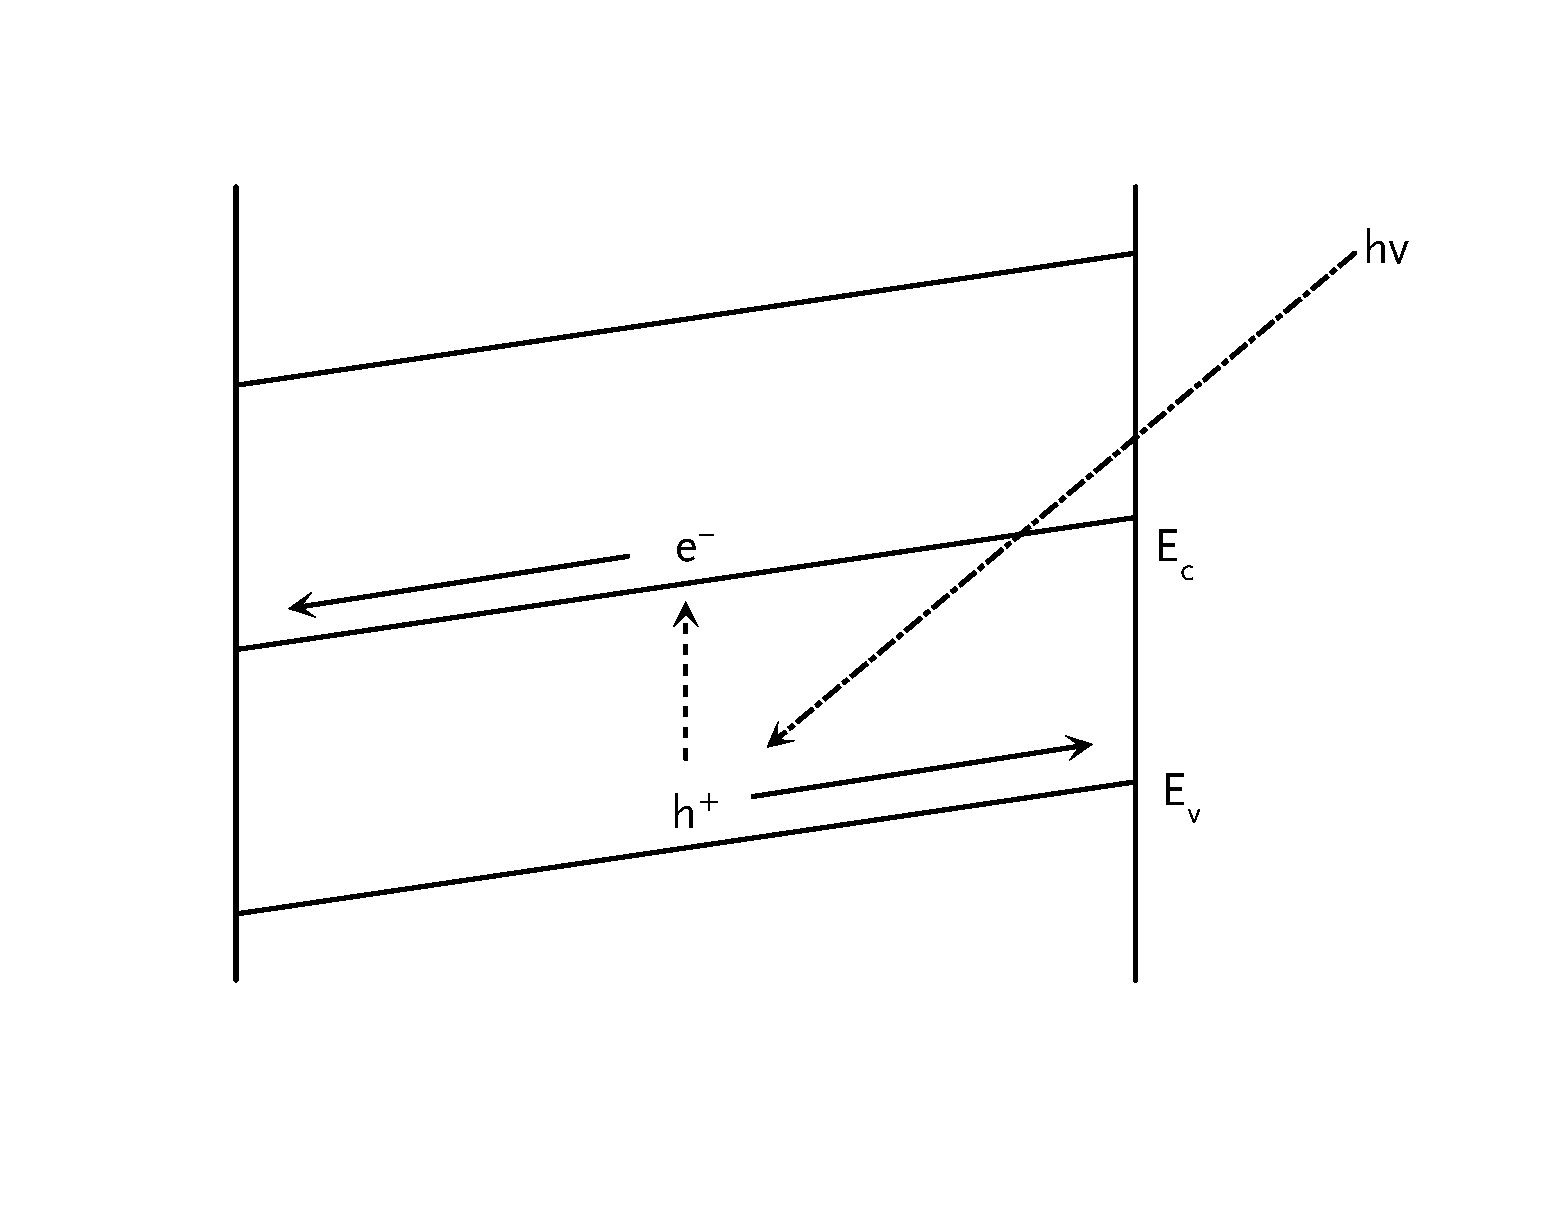
\includegraphics[width=0.8\textwidth]{electronholemovement.pdf}
\caption[Movement of photogenerated charge carriers]{%
	Simplified energy level diagram showing the movement of photogenerated charge carriers in an electric field. The electric field is represented by the sloped bands. Electrons move down on the band to lower energy states, while holes move up.}
\label{fig:electronholemovement}
\end{center}
\end{figure}
%\sidefigure[Movement of photogenerated charge carriers]{%
%	Simplified energy level diagram showing the movement of photogenerated charge carriers in an electric field. The electric field is represented by the sloped bands. Electrons move down on the band to lower energy states, while holes move up.
%	\label{fig:electronholemovement}
%	}{%
%	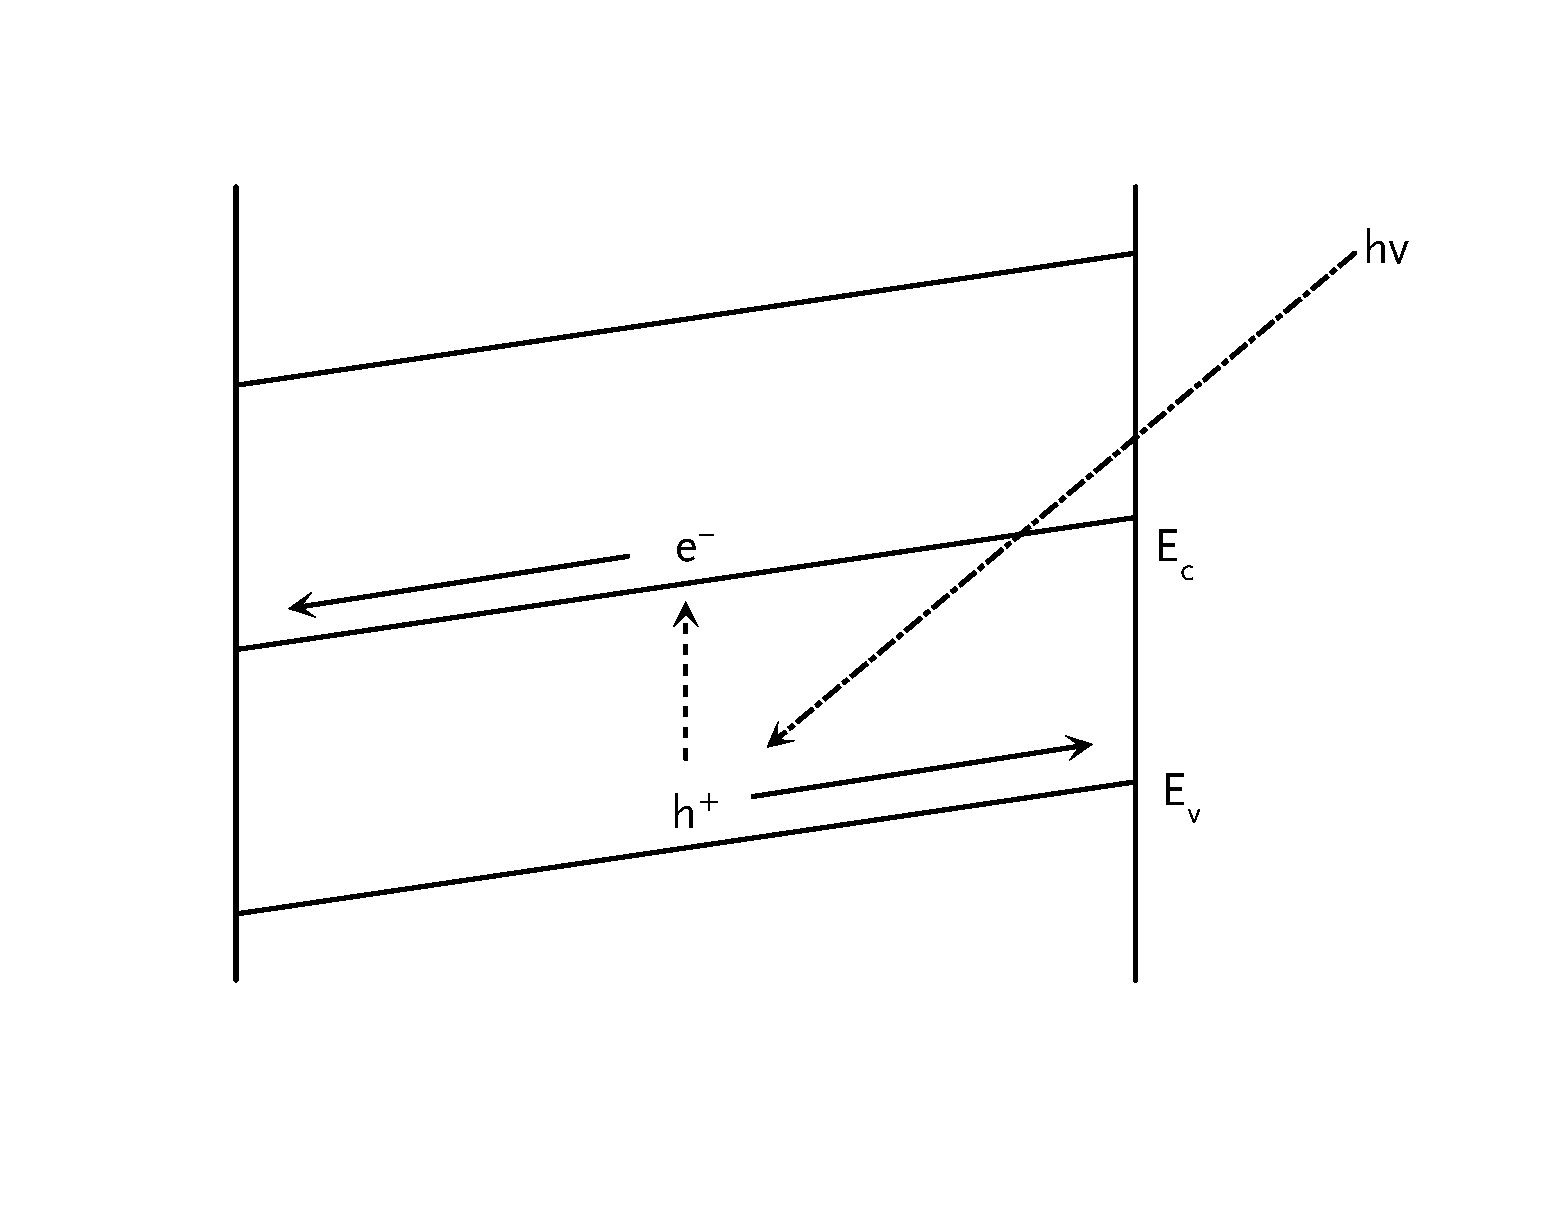
\includegraphics[width=\marginparwidth]{electronholemovement.pdf}
%}{0}


Under the presence of an electric field, electrons and holes are physically separated in a material. The electric field drives electrons and holes in the opposite direction. This is shown schematically in \figureref{electronholemovement}. In simple energy level diagrams such as the one depicted in \figureref{electronholemovement}, electric fields are represented by bands that are angled with respect to the horizontal axis. Electrons are accelerated towards a lower energy state by electric fields, corresponding to traveling ``downhill'' on the band diagram. The reverse is true of holes. Holes are driven ``uphill'' to higher energy states. The presence of electric fields is desirable in the case of photochemistry, as the fields can be engineered to drive electrons or holes to the sample surface, where they can participate in chemical reactions. Electrons and holes that do not reach the surface of the material are eventually lost to recombination, reducing the photochemical efficiency. Heterostructure interfaces are an an established method of generating electric fields within a material. Three possible sources of electric fields in heterostructured interfaces are discussed in this section, including p-n junctions, ferroelectrics, and polar surface terminations. Each of these cases is depicted schematically in \figureref{chargedinterfaces}. 

\begin{figure}

	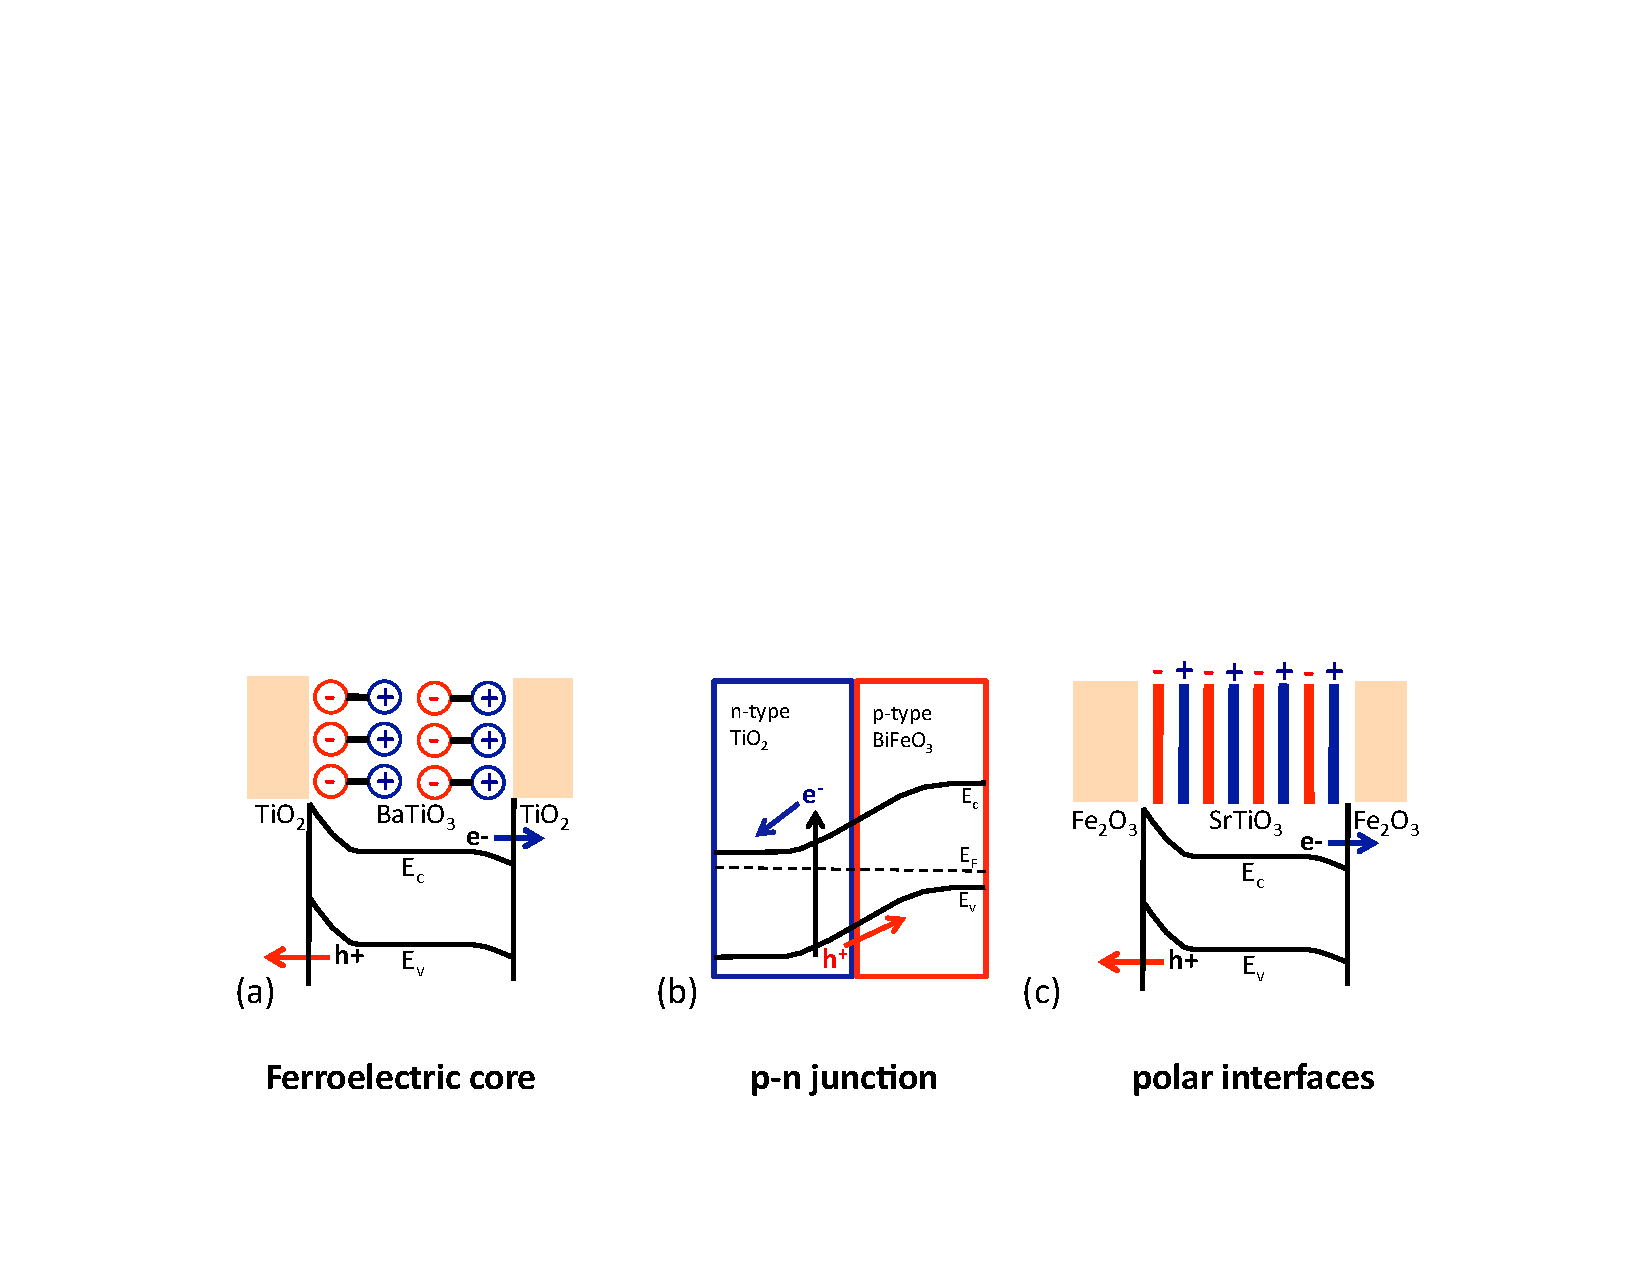
\includegraphics[width=\textwidth]{chargedinterfaces.pdf}
		\caption[Three sources of charged interfaces]{%
			Three sources of charged interfaces. (a) Polarization from a 
			ferroelectric \ce{BaTiO3} core causes electric fields at the 
			surface of a \ce{TiO2} shell. (b) A p-n junction. At the 
			interface, electrons and holes are driven in opposite directions 
			by an electric field as a result of the p-n junction formed by 
			n-type \ce{TiO2} and p-type \ce{BiFeO3}. (c) Uncompensated 
			charge at the interface between a core and film causes electric 
			fields. The charge arises from incompletely compensated polar 
			surface terminations at the interface between \ce{SrTiO3} and 
			\ce{TiO2}.}
	\label{fig:chargedinterfaces}

\end{figure}


\subsection{p-n Junction}
\label{subsec:background.pnjunction}


The presence of a p-n junction has long been known to separate photogenerated charge carriers. A p-n junction arises when a semiconductor with an excess of negative charge carriers (n-type) is placed in contact with a semiconductor with an excess of positive charge carriers (p-type). Excess charge carriers arise in semiconductors as a result of intentional doping with impurity atoms, or as a result of the processing conditions of the material. An intrinsic semiconductor, as in the case of pure silicon, has an equal concentration of electrons and holes. By including a small amount of an impurity element with more or fewer electrons in its valance shell than silicon, the semiconductor can be made p-type or n-type. For example, the inclusion of arsenic in a silicon semiconductor will make the silicon n-type. Arsenic has a five valence electrons, one more than silicon's four, contributing one excess electron for every arsenic atom. If boron, with three valence electrons, is added to pure silicon, the net result is one fewer electron in the material for each boron atom. This ``missing'' electron is termed a hole, and has a positive charge equal in magnitude to the charge on an electron. When studying semiconductors, it is useful to describe the hole as a particle, even through it actually represents the absence of an electron. 

In oxide semiconductors, including all the materials discussed in this document, the bulk oxide often shows p-type or n-type conductivity even in the absence of intentional doping. This arises as a result of the processing conditions. The presence of oxygen vacancies gives rise to n-type oxides, while the presence of metal vacancies gives rise to p-type oxides. The defect reactions corresponding to the formation of oxygen or metal vacancies are:
\begin{align}
	\ce{MO}&\ce{-> M_M + V_O^{\bullet\bullet} + 2e- + 1/2O2_{(g)} \hspace{1em} \text{(Oxygen~vacancy)}} \\
	\ce{MO}&\ce{-> O_O + V_M^{$\prime\prime$} + 2h+ + M_{(g/l/s)} \hspace{1em} \text{(Metal~vacancy)}}
\end{align}
Oxygen vacancies arise through equilibrium with the atmosphere during material fabrication. Increased oxygen partial pressure in during sintering leads to a decrease in oxygen vacancy concentration, and as a result, excess electron concentration. Volatile metal metal elements often lead to metal vacancies during high temperature sintering. For example, bismuth is easily lost to the atmosphere during the sintering of \ce{BiFeO3}, the photochemical properties of which are discussed in this document. The loss of bismuth during sintering leads to its p-type conductivity. Additionally, aliovalent substitution leads to increased charge carriers. For example, the presence of an ion in the $4^{+}$ oxidation state on a $3^{+}$ site leads to on extra free electron.

When n-type and p-type materials are joined, electrons near the junction in the n-type material diffuse into the p-type material, leading to charged regions. The missing electrons in the n-type region leave a region of net positive charge. The excess electrons that have diffused into the p-type material lead to a region of  negative charge. These charged regions, collectively termed the space charge regions, give rise to an electric field. The field drives electrons and holes in opposite directions. If electrons-hole pairs are generated in the region of the electric field, the electrons are driven toward the n-type material, while holes are driven to the p-type material. The formation of the p-n junction and the resulting effect on photogenerated electron hole pairs are shown in \figureref{pnjunction}.

\begin{figure}
	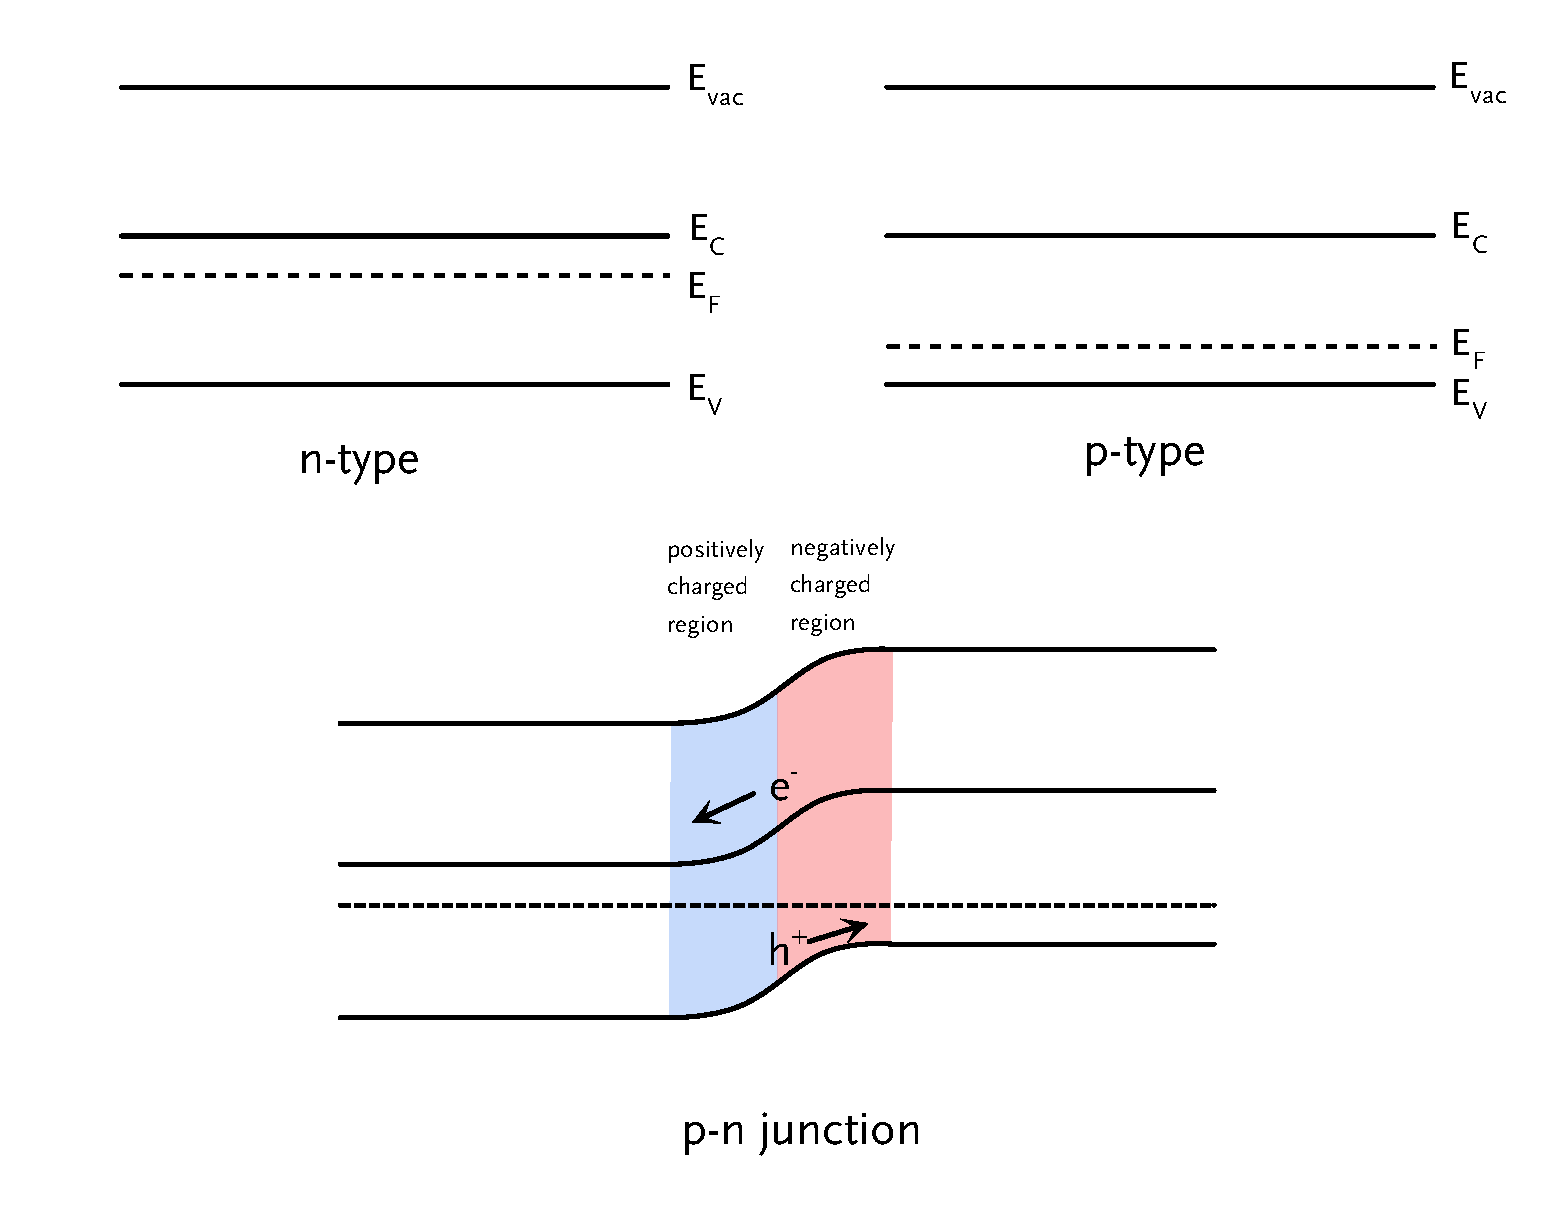
\includegraphics[width=\textwidth]{pnjunction.pdf}
		\caption[The formation of a p-n junction]{%
			The formation of a p-n junction. When an n-type and p-type 
			semiconductor are brought in contact, their Fermi levels 
			align as electrons move from the n-type material into the 
			p-type material. An electric field is created at the 
			interface that drives photogenerated charge carriers in 
			opposite directions.}
	\label{fig:pnjunction}
\end{figure}

The p-n junction is the foundation for conventional solar photovoltaic technology. The photogenerated charges separated by the p-n junction are collected at either end of the device, resulting in a direct current. The same phenomenon also has potential use in photochemical devices, increasing the likelihood of photogenerated charge carriers reaching the surface of the semiconductor, where they can participate the chemical reactions. 


\subsection{Ferroelectric Polarization}
\label{subsec:background.ferroelectric}


Ferroelectrics are a subclass of a group of materials called piezoelectrics. Piezoelectrics are materials that exhibit an electrical polarity under an applied mechanical stress. The reverse is also true; piezoelectric materials deform under an applied electric field. \cite{Lines:1977ug} All piezoelectrics belong to one of the non-centric crystal classes. When a stress is applied to a centrosymmetric crystal, any movement of charge is symmetric, resulting in no net polarization. Charge movement is not symmetric when stress is applied to most non-centrosymmetric crystals, resulting in a net polarization across the crystal. \cite{Lines:1977ug}

Ferroelectric materials exhibit spontaneous polarization below a specific temperature, called the Curie temperature \ce{T_c}, in the absence of an electric field. \cite{Lines:1977ug} Multiple orientational configurations of the polarization vector exist, and an applied electric field can switch the orientation of the polarization vector from one state to another.\cite{Lines:1977ug,Anonymous:7uC1r_sG} As the temperature of a ferroelectric material is lowered below the Curie temperature, different regions of the crystal polarize in each of the different directions. These regions of uniform polarization are called domains.\cite{Lines:1977ug,Anonymous:7uC1r_sG,ForsberghJr:1949vl}

At the surface of the crystal, the termination of the ferroelectric polarization gives rise to a depolarization field. Charge carriers within the crystal can move to the surface to counteract this field. If the field is perfectly compensated by charge carriers, then the energy associated with the depolarization field is zero. However, if the conductivity of the material is low, this compensation could take a very long time, resulting in high energies associated with the depolarization field. However, the formation of domains acts to minimize the energy associated with depolarization fields. The boundaries between domains, across which the polarization vector changes, are called domain walls. Domain walls are usually classified by the angle between the polarization vector on each side of the boundary. As the domain walls stray from the ideal crystal lattice arrangement, a nonzero energy is associated with their formation. The overall domain configuration of the crystal is determined in general by the balancing of the energy gained by reducing the depolarization fields and the energy cost of forming domain walls.

It has been shown that, for ferroelectric materials such as \ce{BaTiO3}, the domain structure effectively promotes photochemical oxidation and reduction on spatially distinct areas of the surface. \cite{Giocondi:2001gz,Burbure:2010go,Giocondi:2003ub,Giocondi:2001bi} Domains with a positive polarization at the surface promote photochemical reduction, while domains with a negative surface polarization promote oxidation. The ferroelectric polarization acts to bend the bands at the surface. The positive polarization bends the bands downward, driving electrons to the surface. The negative polarization bends the bands upward, driving holes to the surface. This effect is shown schematically in \figureref{ferroelectric}. Similar effects have also been observed in ferroelectric \ce{Pb(Zr_{x}T_{1-x})O3} (\abbr{PZT}) and \ce{LiNbO3}.\cite{Hanson:2006bq,Kalinin:2002iw,Tiwari:2009jv}

\begin{figure}
	\centerline{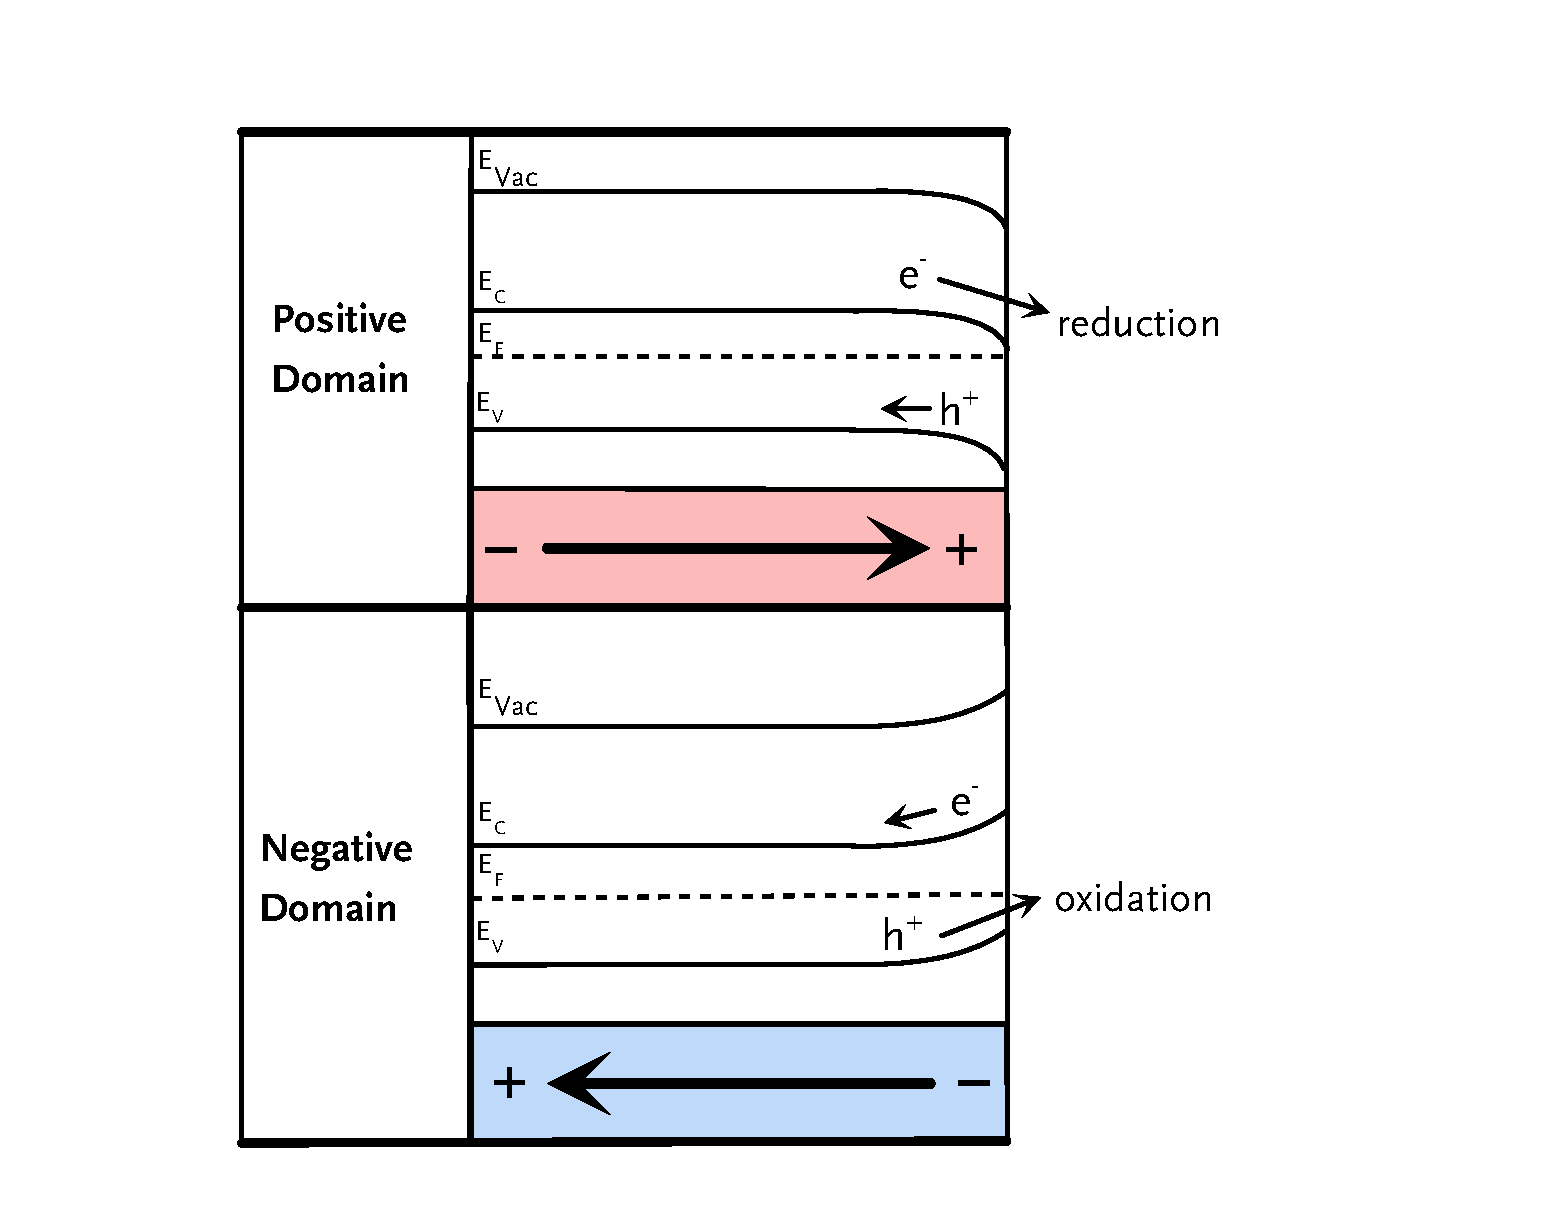
\includegraphics[width=0.8\textwidth]{ferroelectric.pdf}}
	\caption[Band bending at the surface of ferroelectric domains]{%
		Band bending at the surface of ferroelectric domains. A positive 
		domain has the bands bent downward at the surface, favoring 
		reduction. A negative domain has the band bend upwards, favoring 
		oxidation.}
	\label{fig:ferroelectric}
\end{figure}

By driving charge carriers in opposite directions, the ferroelectric fields reduce the recombination rates of electron-hole pairs generated in the space charge region near the surface of the ferroelectric. Additionally, because oxidation and reduction are occurring on distinct areas of the sample surface, the ferroelectric fields are hypothesized to reduce the rate of back reaction of intermediate products in the water splitting process. Burbure\cite{Burbure:2010go,Burbure:2006cq,Burbure:2010ti} demonstrated that the spatial separation of oxidation and reduction from ferroelectric domains persists, even when a thin film of \ce{TiO2} was deposited on \ce{BaTiO3}. This phenomenon suggest the possibility of increased photochemical efficiency through the inclusion of ferroelectric interfaces.


\subsection{Polar Terminations}
\label{subsec:background.polarterms}


\begin{figure}
\begin{center}
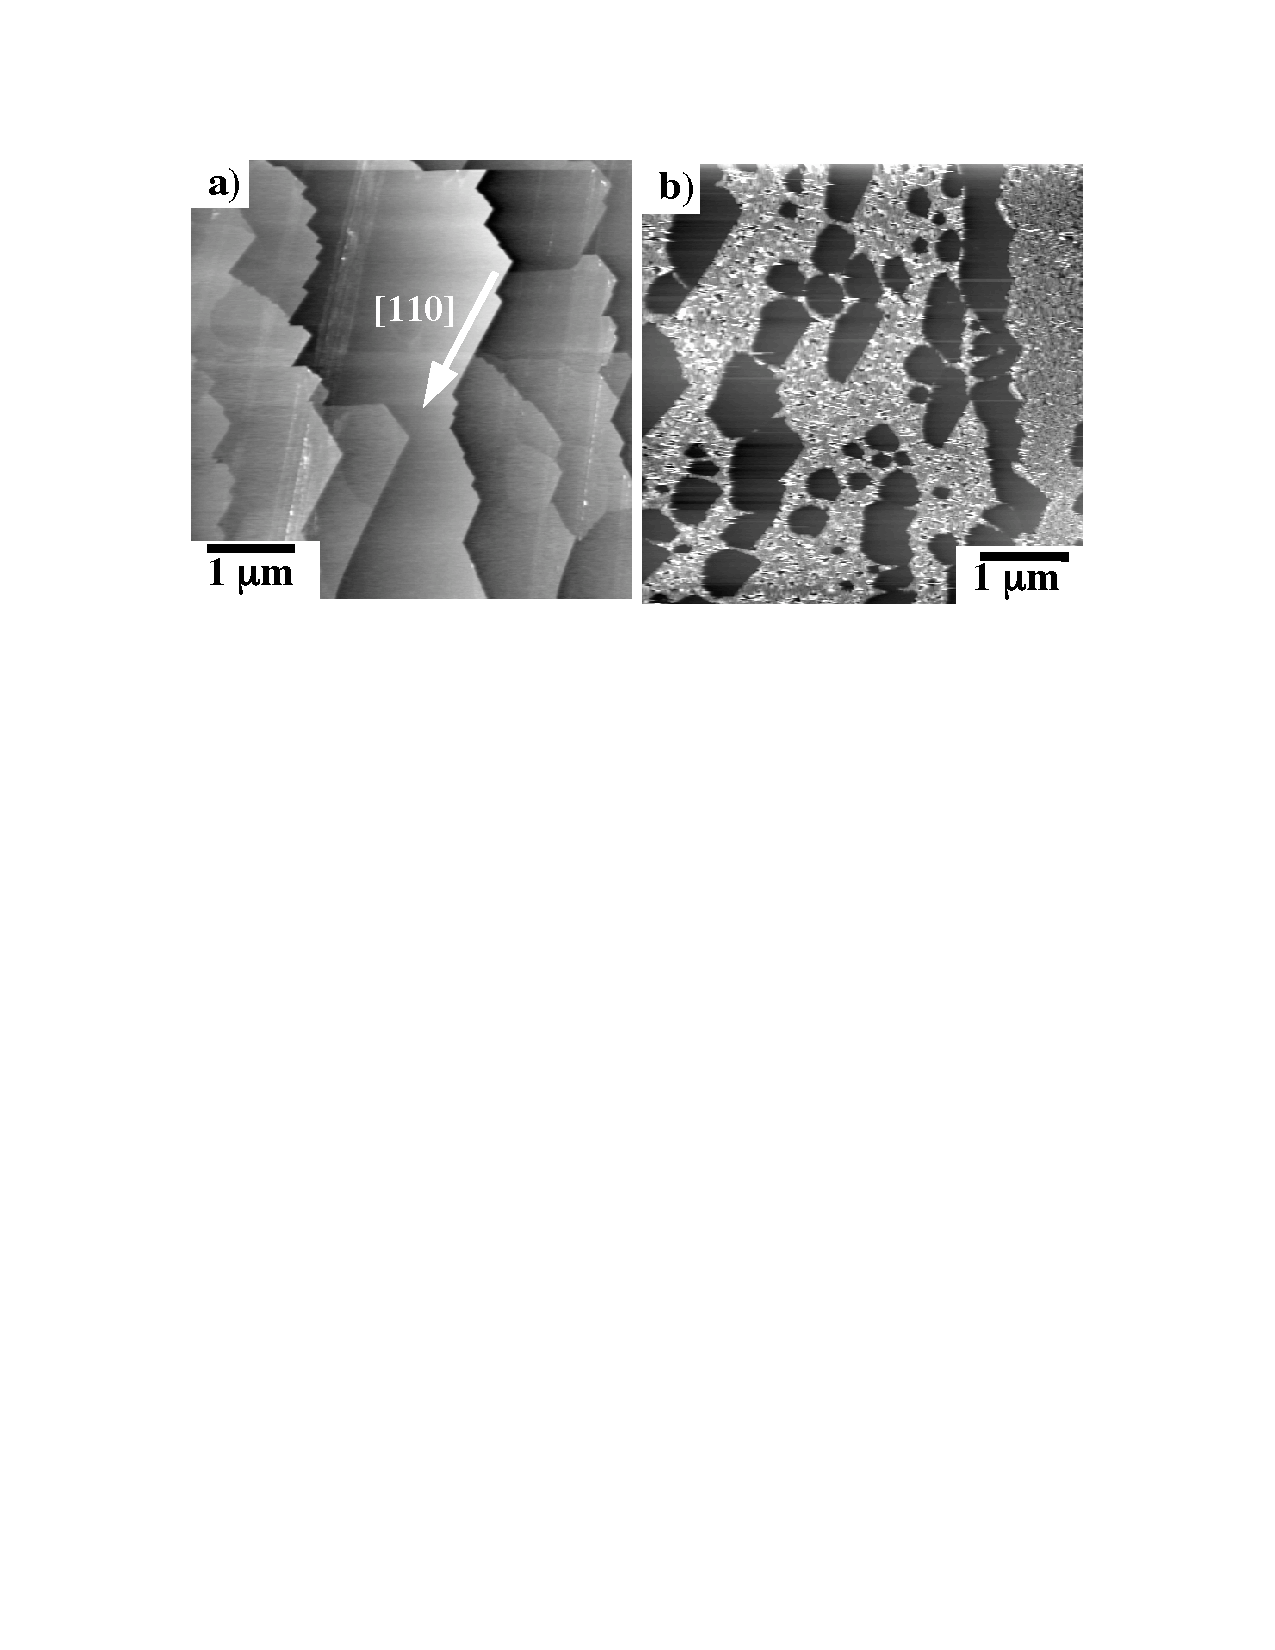
\includegraphics[width=0.8\textwidth]{giocondi.pdf}
\caption[Surface of an annealed \ce{SrTiO3} (111) single crystal]{%
	The surface of an annealed \ce{SrTiO3} (111) single crystal before 
	(a) and after (b) reaction with \ce{AgNO3}. The silver is preferentially 
	deposited on certain faces, corresponding to surfaces of different 
	polar terminations.\cite{Giocondi:2003wc}}
\label{fig:giocondi}
\end{center}
\end{figure}
%\sidefigure[Surface of an annealed \ce{SrTiO3} (111) single crystal]{%
%	The surface of an annealed \ce{SrTiO3} (111) single crystal before 
%	(a) and after (b) reaction with \ce{AgNO3}. The silver is preferentially 
%	deposited on certain faces, corresponding to surfaces of different 
%	polar terminations.\cite{Giocondi:2003wc}
%	\label{fig:giocondi}
%	}{%
%	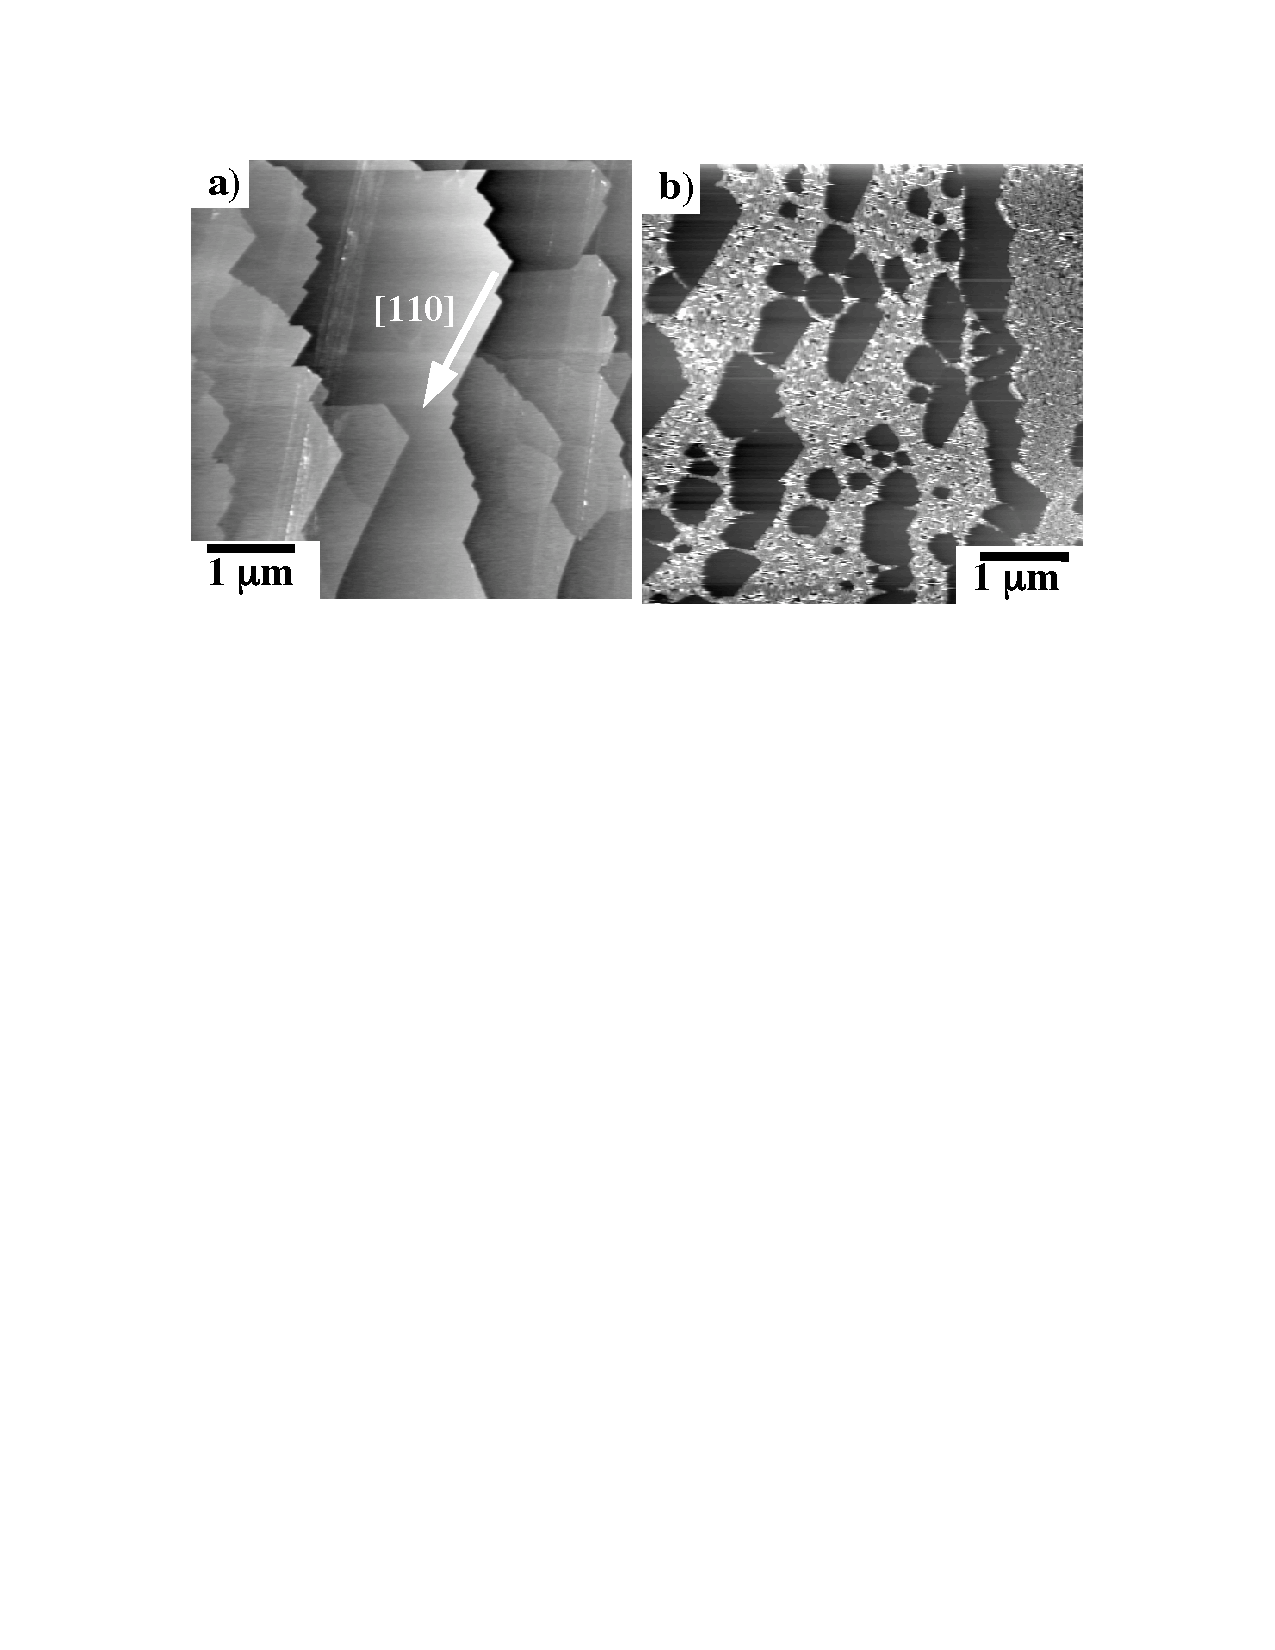
\includegraphics[width=\marginparwidth]{giocondi.pdf}
%}{-2}
Giocondi\cite{Giocondi:2003wc} discovered that polar surface terminations can also result in spatially selective photochemical reactivity on the surface of \ce{SrTiO3}. \figureref{giocondi} shows the surface of a (111) \ce{SrTiO3} single crystal before and after photochemical reaction with aqueous silver nitrate. The bright areas on the surface after reaction correspond to the reduced solid silver reaction product. The silver does not cover the entire surface. Instead, it appears as regions of total coverage and regions of no coverage. The shapes of these regions appear similar to the shapes of the terraces before reaction. Giocondi attributed this spatially selective reaction to the two possible surface terminations of the (111) \ce{SrTiO3} surface. As discussed in more detail in \sectionref{subsubsec:background.sto} on \ce{SrTiO3} crystallography, (111) \ce{SrTiO3} surfaces are terminated by either \ce{SrO3^{4-}} or \ce{Ti^{4+}} layers. After measuring the step heights between the terraces on the clean surface, it was determined that regions of similar reactivity correspond to terraces separated by an even multiple of the spacing between lattice planes. Areas of differing reactivity were separated by an odd multiple. From this information, it was concluded that the areas of high reactivity shared the same termination, and all nonreactive areas shared the other termination.

It was hypothesized that the charge at these surfaces could lead to the presence of a space charge region at the surface, similar to that for ferroelectric polarization. Terraces with a \ce{SrO3^{4-}} termination have a negative surface charge, associated with a upward band bending at the surface. \ce{Ti^{4+}} terminated surfaces have a positive surface charge, leading to negative band bending. This hypothesis is illustrated schematically in \figureref{polarterminations}. Up to this point, the effect of polar surface terminations on the photochemical reactivity of supported films has not been tested. The effect of the polar surface terminations of (111) \ce{SrTiO3} on the reactivity of hematite films is reported in this document.
\begin{figure}
	\centerline{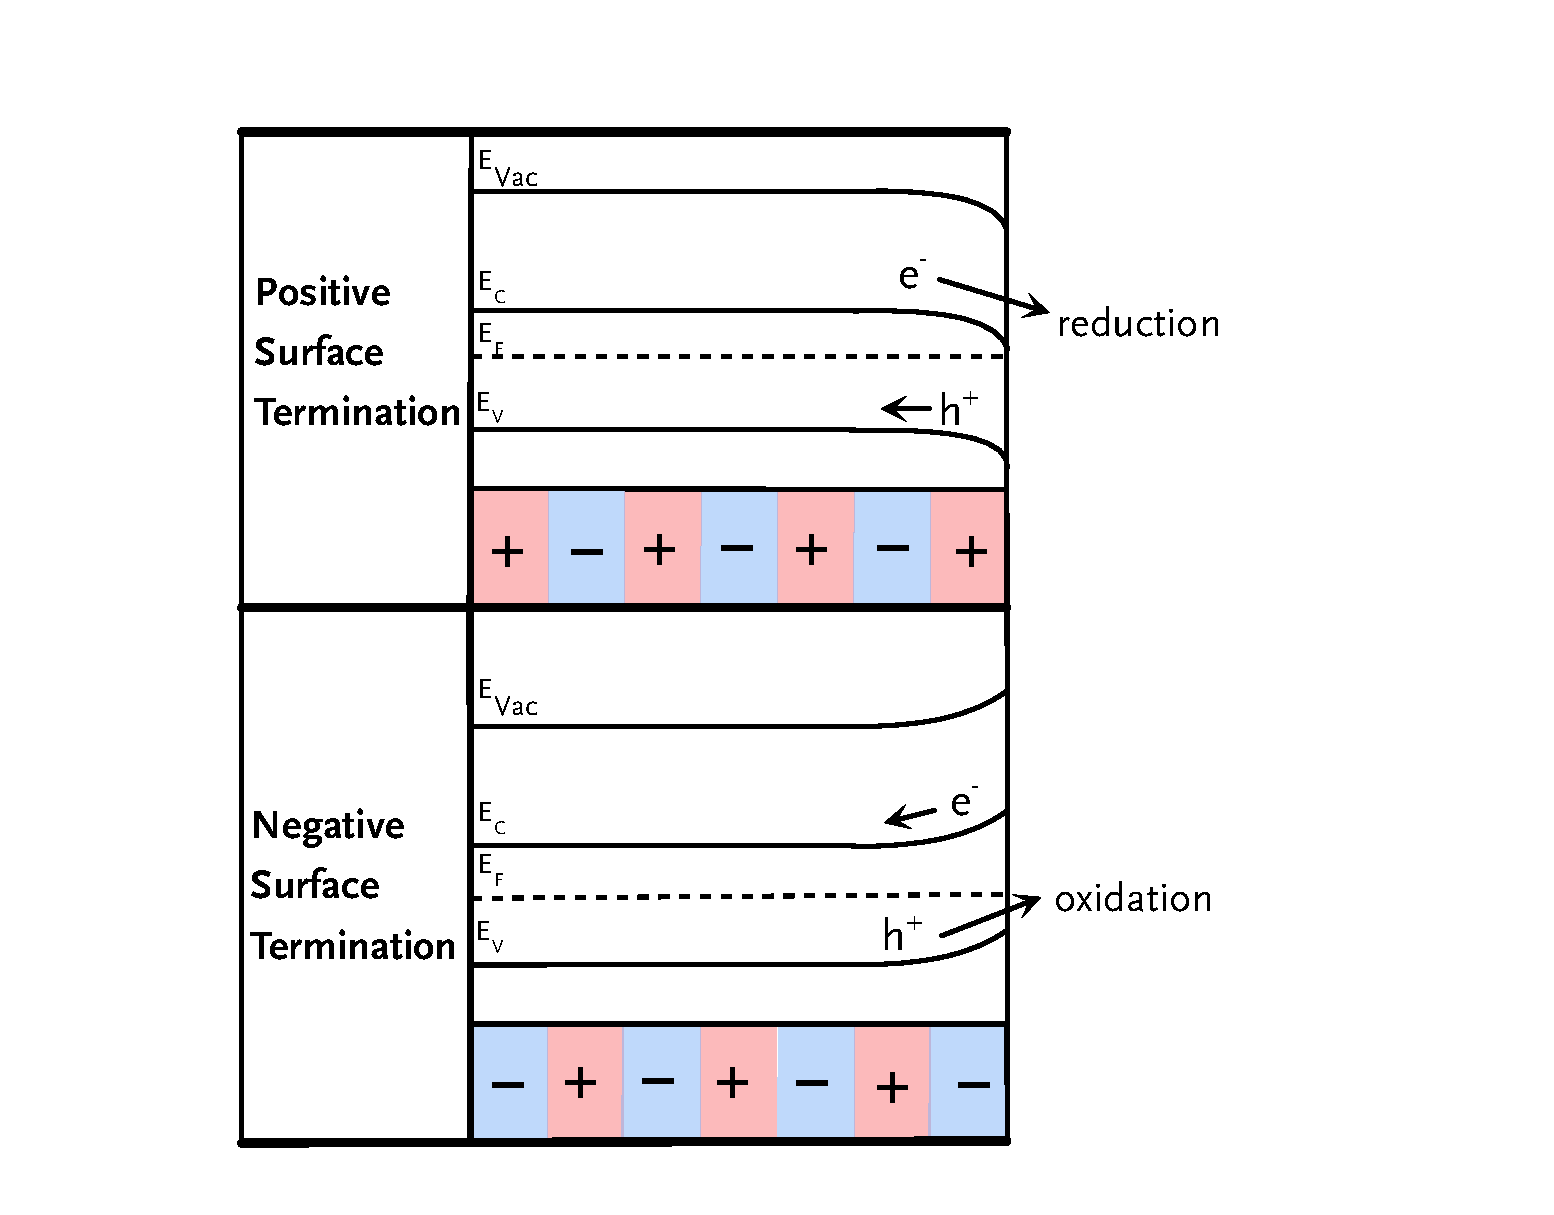
\includegraphics[width=0.8\textwidth]{polarterminations.pdf}}
	\caption[Band bending arising from polar surface terminations]{%
		Band bending at the surface of an orientation with polar surface 
		terminations. A positive surface termination bends the bands 
		downward, favoring reduction. A negative surface charge bends the 
		bands upward, favoring oxidation.}
	\label{fig:polarterminations}
\end{figure}


\section{Epitaxy}
\label{sec:background.epitaxy}


Epitaxy refers the ordered growth of new solid film phase on an existing solid material.\cite{Opel:2012ge,Herman:2004to,Hooks:2001vy} During epitaxial growth, the  film phase and orientation can be controlled through proper choice of substrate and processing conditions. The periodic lattice of the substrate drives the film to adopt a lattice with similar lattice parameters. Epitaxial film growth is an important aspect of electronic and optical technologies.

\begin{figure}
\begin{center}
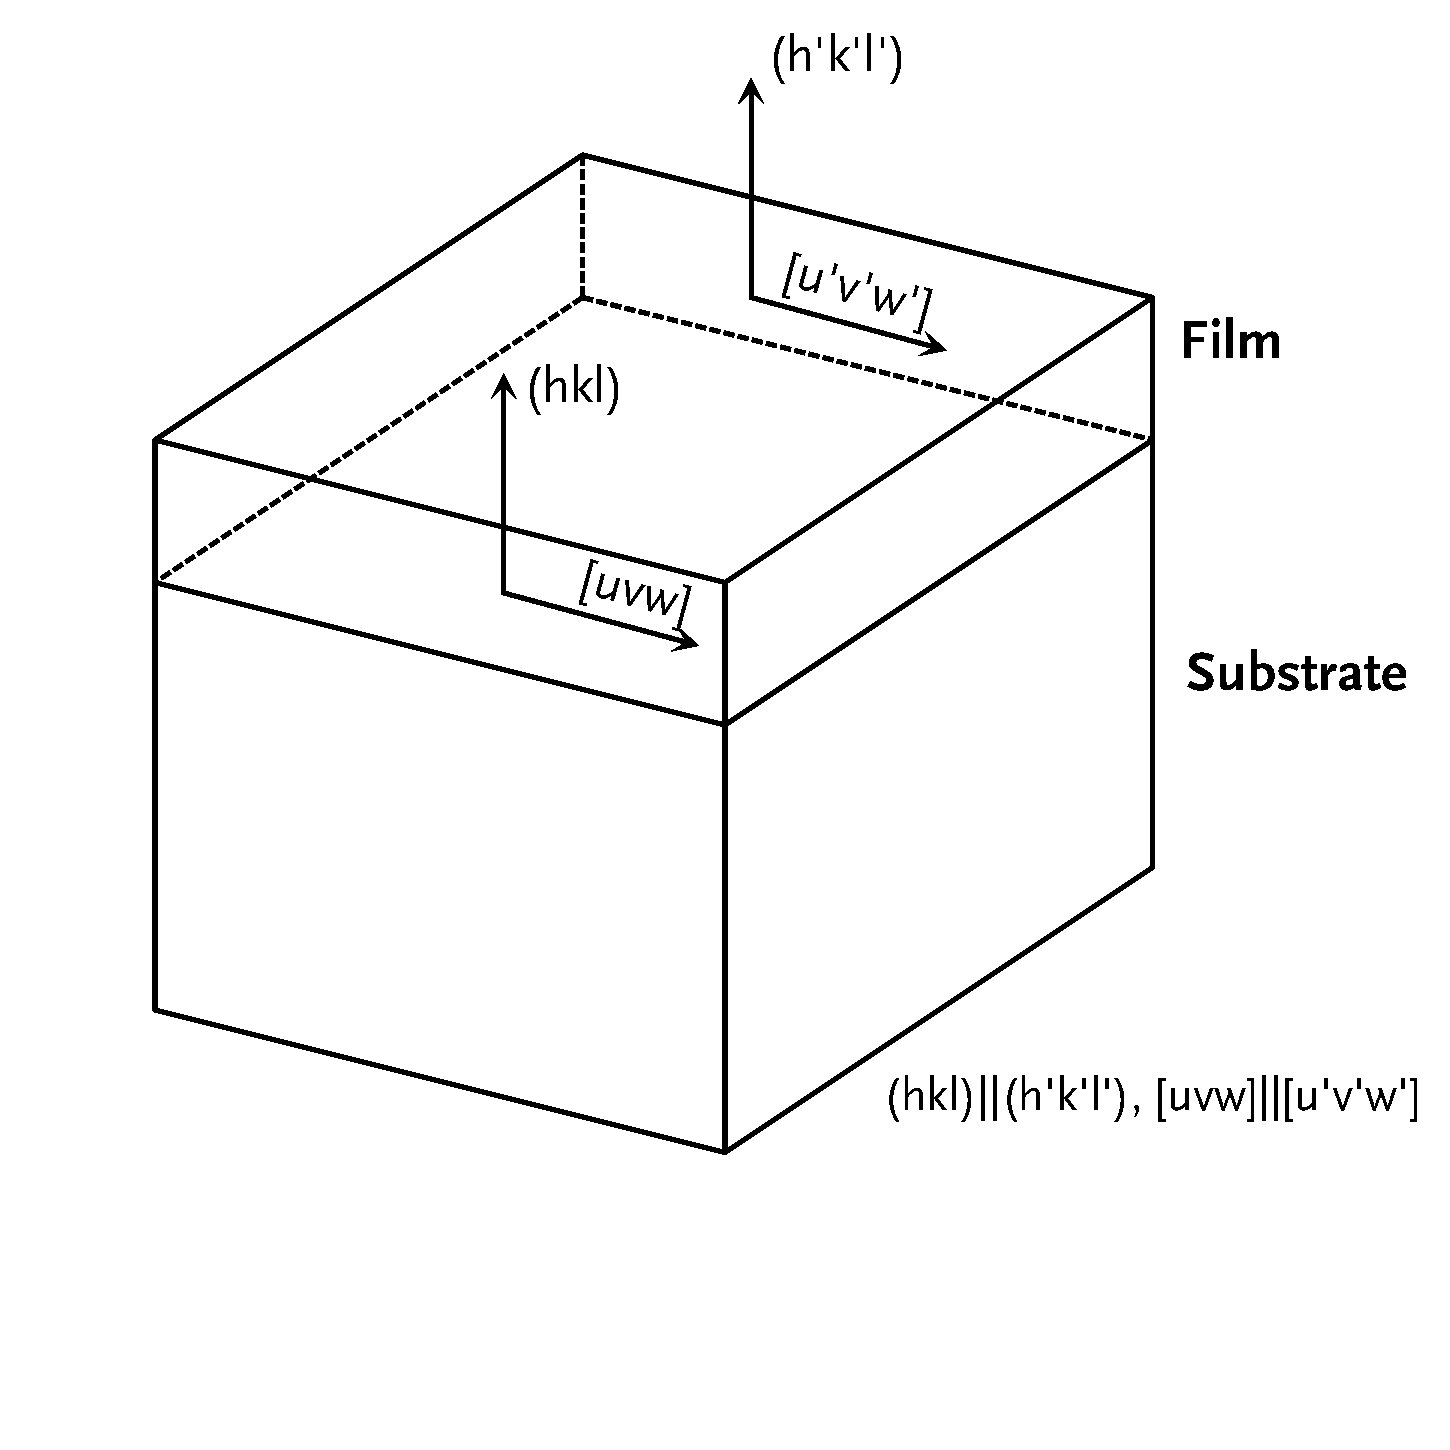
\includegraphics[width=0.7\textwidth]{epitaxy.pdf}
\caption[Orientation relationships in epitaxy]{%
	Diagram showing the sets of parallel directions that describe epitaxial 
	growth. The planes of the film and substrate parallel to the sample surface
	make up one pair. A direction within that plane makes up the second pair. }
\label{fig:epitaxy}
\end{center}
\end{figure}
%\sidefigure[Orientation relationships in epitaxy]{%
%	Diagram showing the sets of parallel directions that describe epitaxial 
%	growth. The planes of the film and substrate parallel to the sample surface
%	make up one pair. A direction within that plane makes up the second pair. 
%	\label{fig:epitaxy}
%	}{%
%	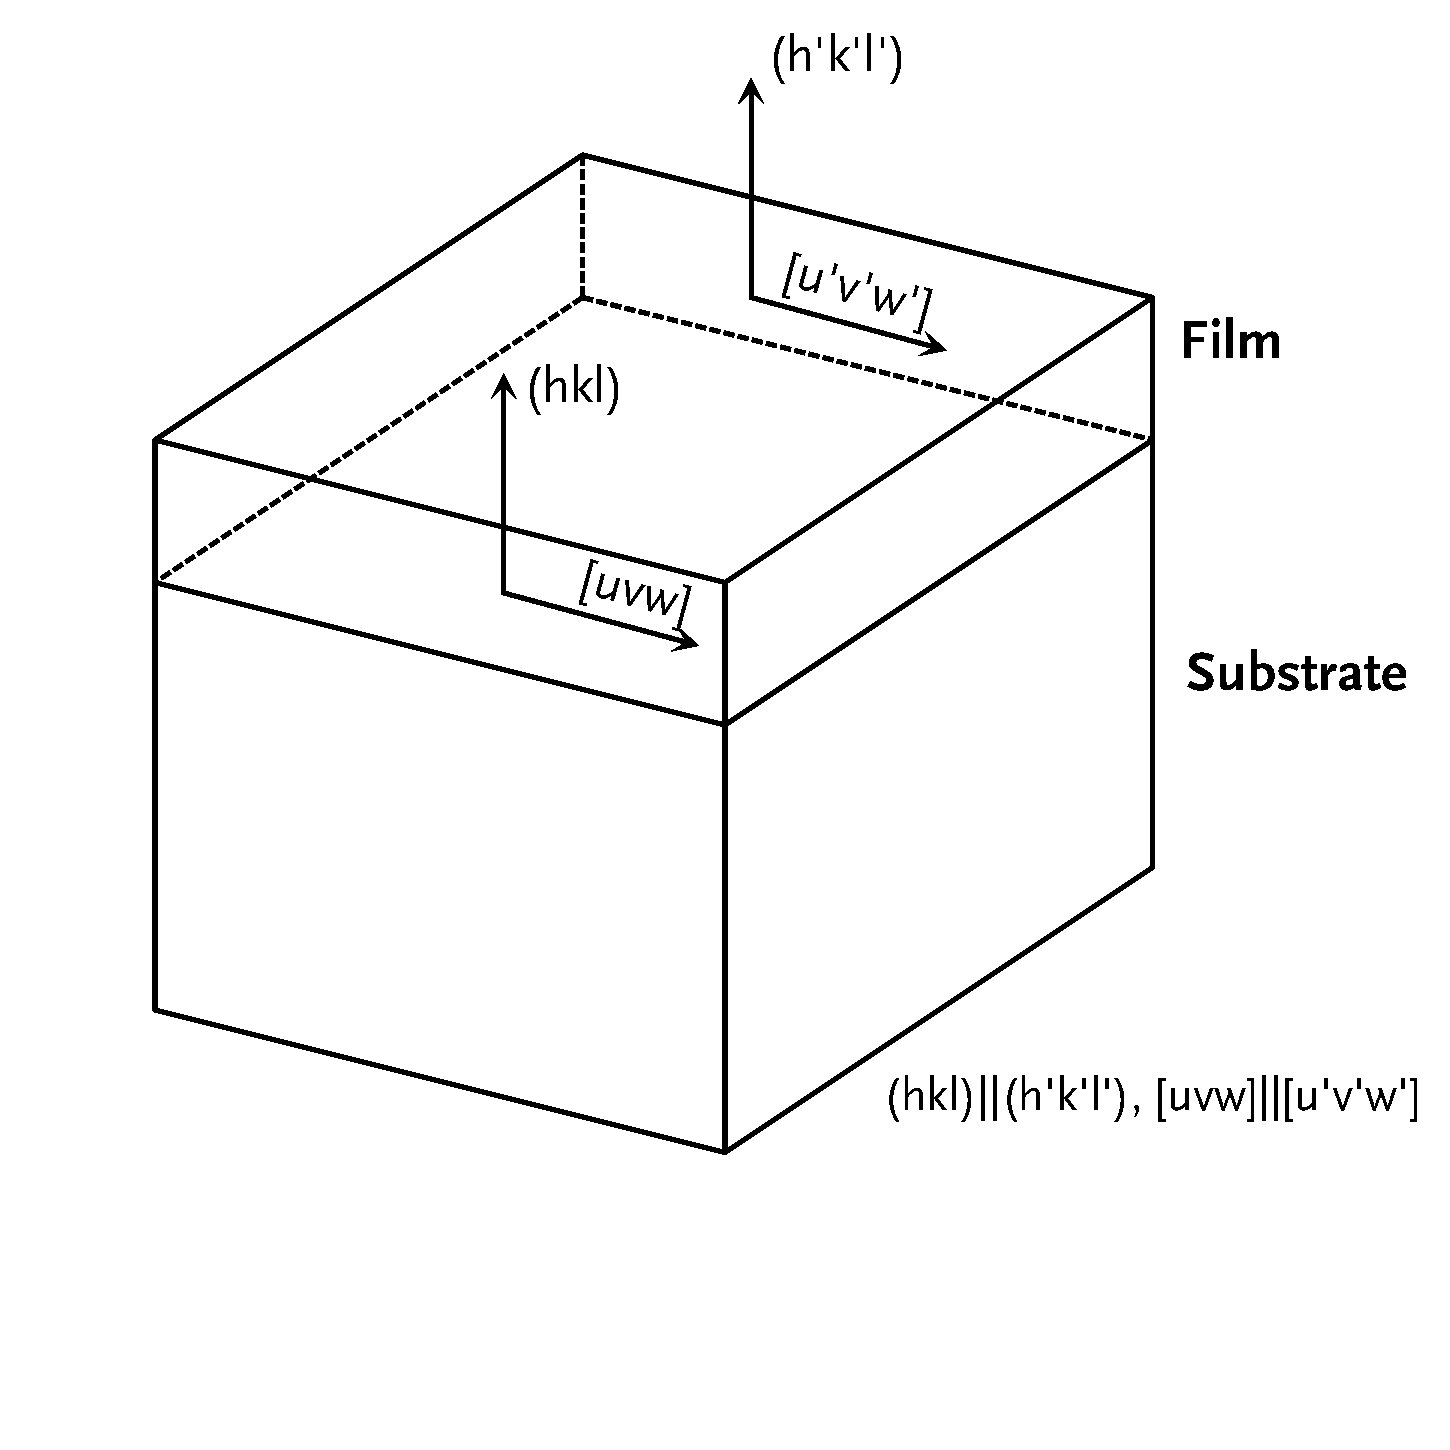
\includegraphics[width=\marginparwidth]{epitaxy.pdf}
%}{-15} % Last argument is number of lines to move up or down
Depending on the nature of the materials involved in film growth, the type of epitaxy can be termed homoepitaxy or heteroepitaxy. Homoepitaxy refers to growth of the same material as the substrate. When the film material is different from the substrate material, the process is called heteroepitaxy. For example, this document reports on heteroepitaxial hematite films grown on perovskite substrates. Epitaxial growth is characterized by a consistent orientation relationship between the film and the substrate. This relationship is described by two orthogonal pairs of parallel directions. Generally, the first pair is the set of normals to the planes parallel to the sample surface in both the film and the substrate. The second pair is two parallel directions within that plane (one in the substrate, one in the film). 

Predictions of epitaxial growth and the resulting orientation relationships typically look at a 2\textsc{D} analysis of the surface lattice parameters. If possible, the film material is energetically stabilized by forming a face and orientation that closely matches the substrate lattice parameter. The difference between the film and substrate lattice parameter is called the lattice misfit, and is given by 
\begin{equation}
f=\frac{a_{f}-a_{s}}{a_{s}},
\end{equation}
where $a_{f}$ is the film lattice parameter and $a_{s}$ is the substrate lattice parameter.\cite{Opel:2012ge} When the lattice mismatch $f$ is zero, the film lattice parameter is equal to the substrate lattice parameter and the film is unstrained. When $f$ is less than zero, the film lattice parameter is smaller than the substrate lattice parameter and an epitaxial film will exhibit tensile in plane strain and compressive out of plane strain. When the reverse is true and $f$ is greater than zero, the film experiences compressive in plane strain and tensile out of plane strain. As the film grows thicker, misfit dislocations can be introduced to the lattice, reducing the strain of the film. Above a certain thickness d$_{c}$ specific to the film-substrate system, the film is relaxed, and additional layers are generally unstrained, excepting sources of local strain such as misfit and threading dislocations. Each of these cases is illustrated schematically in \figureref{filmgrowth}.
\begin{figure}
	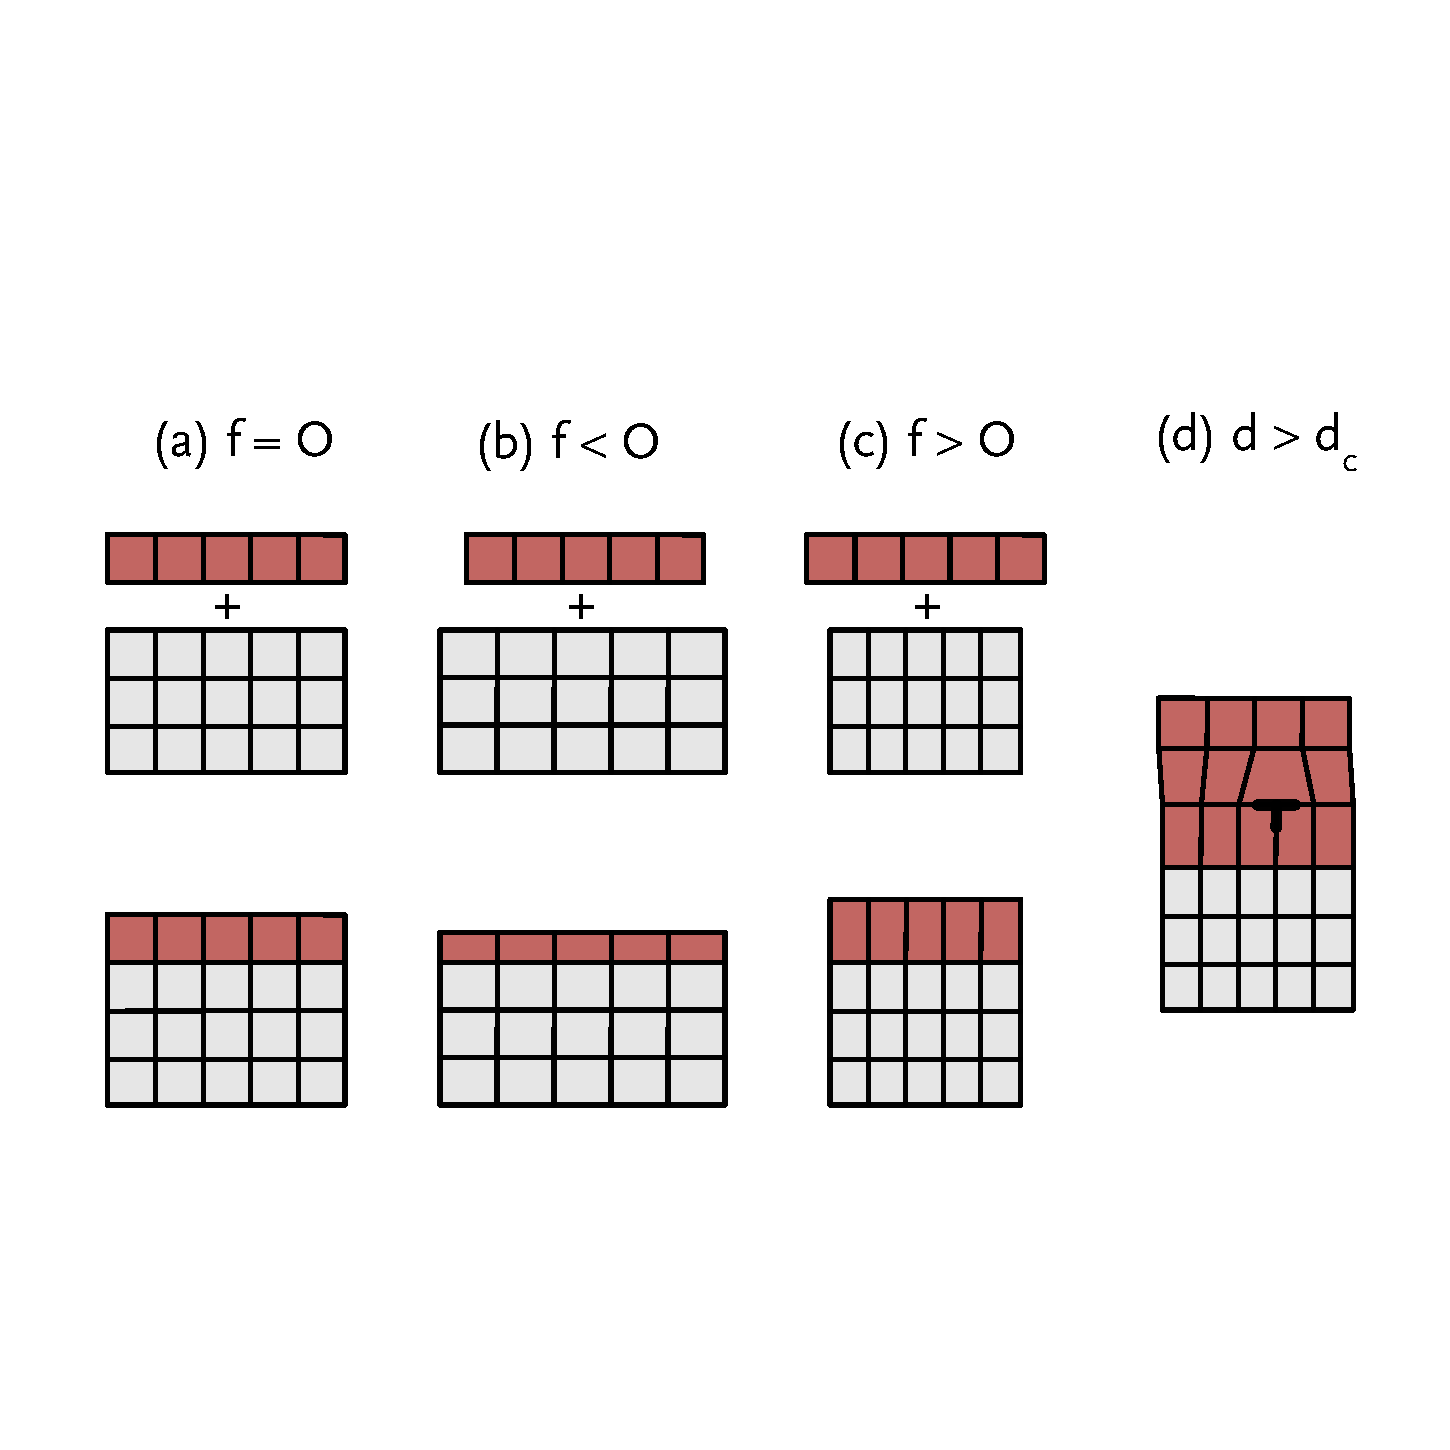
\includegraphics[width=\textwidth]{filmgrowth.pdf}
		\caption[Strain in thin film growth]{%
			(adapted from Opel\citep{Opel:2012ge}) Effect of lattice mismatch 
			on epitaxial growth and strain.
			When the film lattice parameter equals the substrate, as in (a),
			the film is unstrained. A smaller film lattice parameter (b) or
			larger film lattice parameter (c) than the substrate results in
			a strained film. (d) As the film grows thicker, dislocations appear
			in the lattice, reducing the strain state of the film.}
	\label{fig:filmgrowth}
\end{figure}

In this document, the nature of epitaxy for hematite film growth on various oxide substrates is explored. Initially, epitaxial growth was obtained on favorable substrates such as \ce{Al2O3} or (111)-oriented \ce{SrTiO3} which are isostructural or have an isostructural surface lattice respectively. Then film growth, epitaxy and orientation relationships were observed for more unconventional substrates, including (001)-oriented \ce{SrTiO3}, which has a different surface structure than \ce{Fe2O3} or polycrystalline substrates, which expose complex high index surface planes. Film growth on these high index planes, and the resulting orientation relationships are reported in this document.

\section{Crystallography}
\label{sec:background.crystallography}


Crystal structure plays an important role in the photochemical reactivity and epitaxy of oxide materials. The following sections give a brief overview of the crystallographic properties of the materials mentioned in this document.

\subsection{Hematite}
\label{subsec:background.hematite}

\begin{figure}
\centering
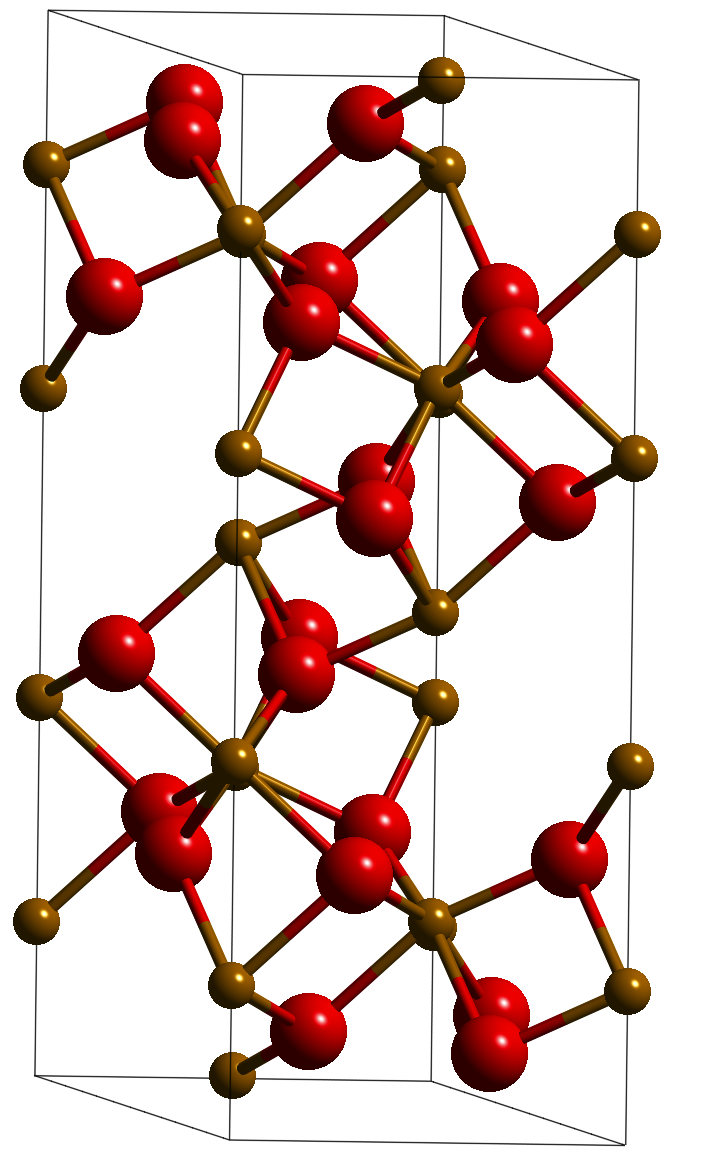
\includegraphics[width=0.4\textwidth]{hematitecell.png}
\caption[Hexagonal hematite unit cell]{%
	The hematite hexagonal unit cell. Red atoms represent oxygen, and brown atoms represent iron.  The structure is formed by hexagonal close packed oxide ions stacked along [0001] with ferric ions in two thirds of the octahedral interstices.}
\label{fig:hematitecell}

\end{figure}
%\sidefigure[Hematite hexagonal unit cell]{%
%	The hematite hexagonal unit cell. Red atoms represent oxygen, and brown atoms represent iron.  The structure is formed by hexagonal close packed oxide ions stacked along [0001] with ferric ions in two thirds of the octahedral interstices.
%	\label{fig:hematitecell}
%	}{%
%	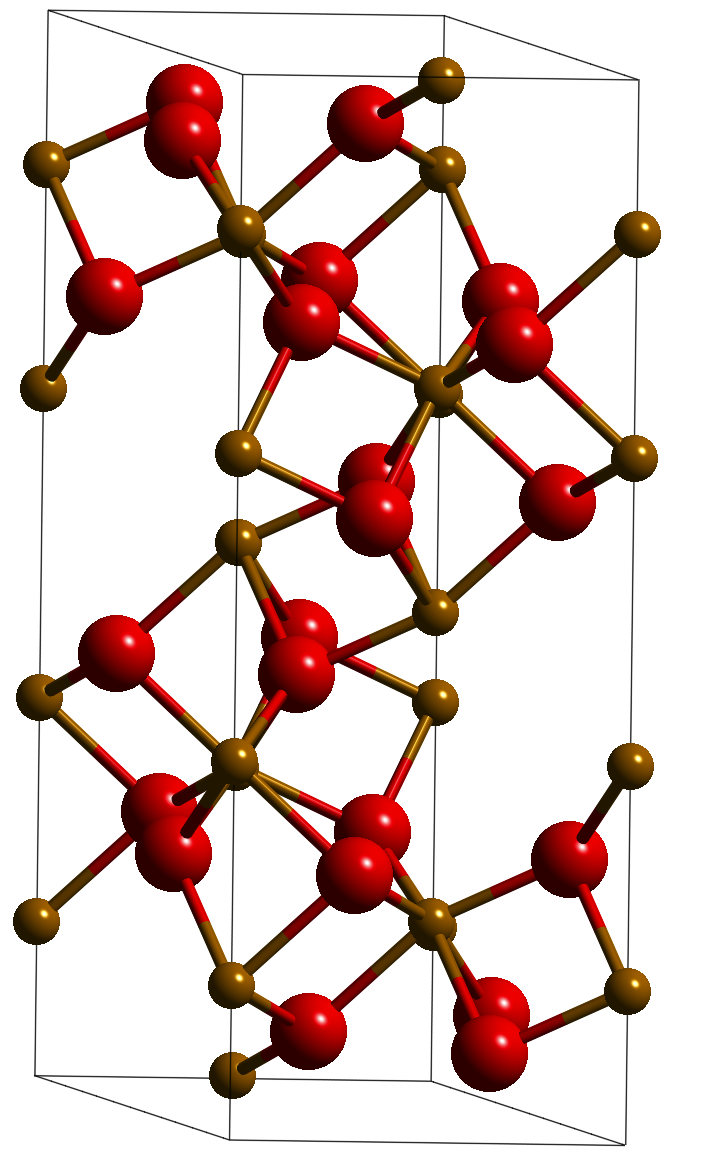
\includegraphics[width=\marginparwidth]{hematitecell.png}
%}{-18}

Hematite, \textalpha-\ce{Fe2O3}, is a promising material for use as a photolysis catalyst because it has a band gap of about 2.2~eV, which lies well into the visible spectrum.\cite{Lin:2011kw} This band gap is also larger than the minimum required to split water, 1.23~eV. Additionally, \ce{Fe2O3} is inexpensive, readily available, chemically stable in aqueous environments, and doesn't contain environmentally hazardous elements. Hematite has been widely studied for photochemical purposes,\cite{Sivula:2011cc} including as powders,\cite{GONDAL:2004df} thin films,\cite{Cao:2010dm} and as a heterojunction component.\cite{Luo:2006kg,Wang:2007fp} However, the efficiency of \ce{Fe2O3} as a photocatalyst is thought to be limited by low hole mobility and short carrier lifetimes.\cite{Sivula:2011cc} Incorporating semiconductors in heterostructures to improve photochemical activity is widely reported.\cite{Maruska:1979tr} 

In this document, the photochemical behavior of \ce{Fe2O3} films on single crystal and polycrystalline substrates is discussed. Details of \ce{Fe2O3} film growth on these substrates are also reported, including the orientation relationships between \ce{Fe2O3} films and perovskite substrates. The corundum type structure of the hematite unit cell is shown in \figureref{hematitecell}. The structure is formed by layers of hexagonal-close-packed oxygen ions stacked along the [0001] direction, with iron(III) ions in two-thirds of the octahedral interstices. This arrangement is of importance when considering the heteroepitaxy of \ce{Fe2O3} films on perovskite substrates, presented in this document. 

\subsection{Perovskites}\label{subsec:background.perovskites}

The perovskite structure is formed by many materials with the formula \ce{ABO3}, where A and B are metal cations, and the A cation is significantly larger than the B cation.\cite{Bhalla:2000ku} The cell takes the form of a cubic cell with the larger A cation sitting on the cubic P lattice sites. The smaller B cation occupies the body centered position of the cubic cell, while the O anions occupy the face centers of the unit cell. This configuration can be described as \ce{AO3} forming a cubic close packed network with B cations in one quarter of the octahedral interstices.

In addition to the prototypical cubic structures, perovskites are also found in a variety of distorted cubic lattices. Common perovskite distortions give rise to tetragonal, orthorhombic, and rhombohedral unit cells. The distortion of the unit cell gives rise to materials with many interesting properties, including ferroelectricity and ferromagnetism. Perovskite materials are widely studied\cite{Bhalla:2000ku} for applications in electronic devices,\cite{Kingon:2000wa} fuel cells,\cite{Zhu:2003jz,Jiang:2008fb} gas sensors,\cite{Fergus:2007tm} superconductivity,\cite{Murphy:1987wc} and catalysis.\cite{Lombardo:1998uv}

\subsubsection{Strontium Titanate}\label{subsubsec:background.sto}

\begin{figure}
\begin{center}
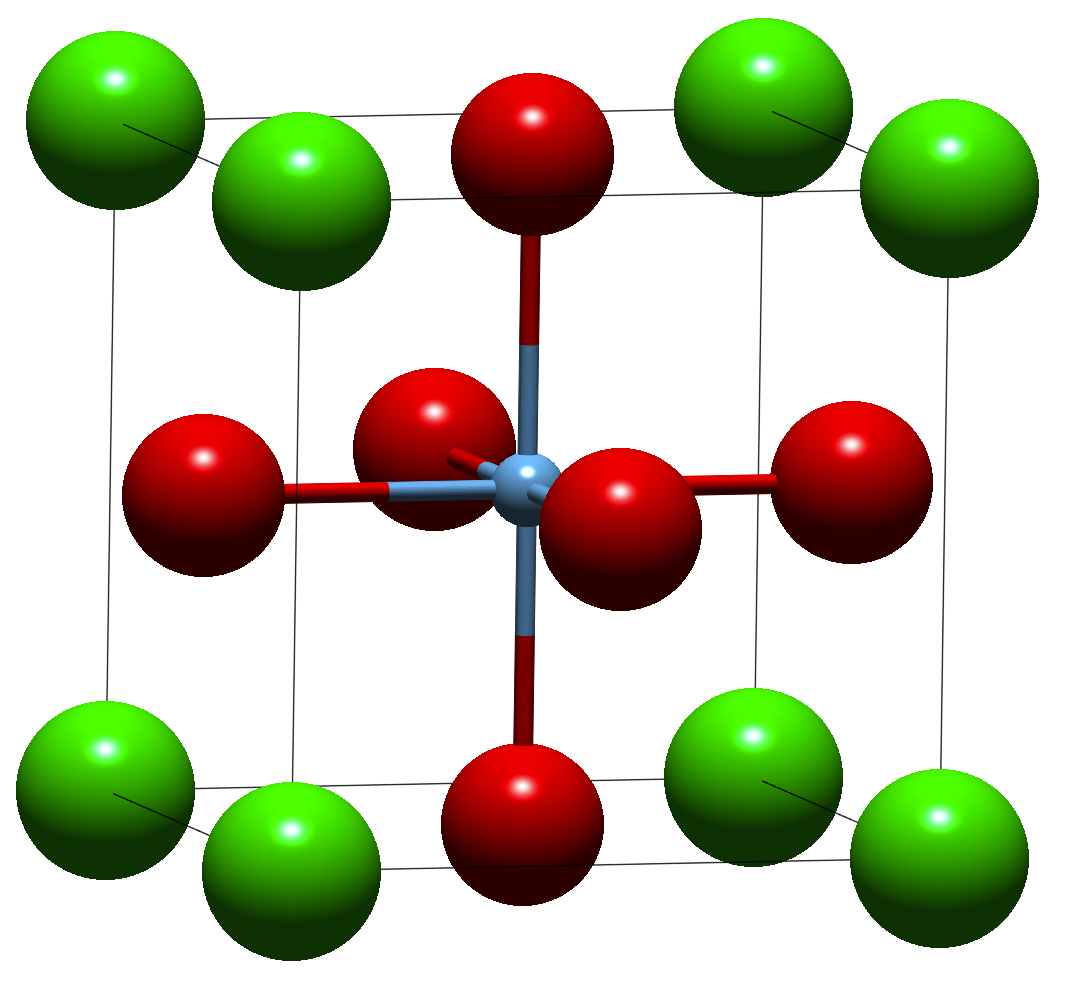
\includegraphics[width=0.4\textwidth]{stocell.png}
\caption[Cubic \ce{SrTiO3} unit cell]{%
	The cubic \ce{SrTiO3} unit cell. The cell takes the form of a 
	cubic cell with the larger Sr cation (green) sitting on the 
	cubic P lattice sites. The smaller Ti cation (blue) occupies 
	the body centered position of the cubic cell, while the O anions 
	(red) occupy the face centers of the unit cell.}
\label{fig:stocell}
\end{center}
\end{figure}
%\sidefigure[Cubic \ce{SrTiO3} unit cell]{%
%	The cubic \ce{SrTiO3} unit cell. The cell takes the form of a 
%	cubic cell with the larger Sr cation (green) sitting on the 
%	cubic P lattice sites. The smaller Ti cation (blue) occupies 
%	the body centered position of the cubic cell, while the O anions 
%	(red) occupy the face centers of the unit cell.
%	\label{fig:stocell}
%	}{%
%	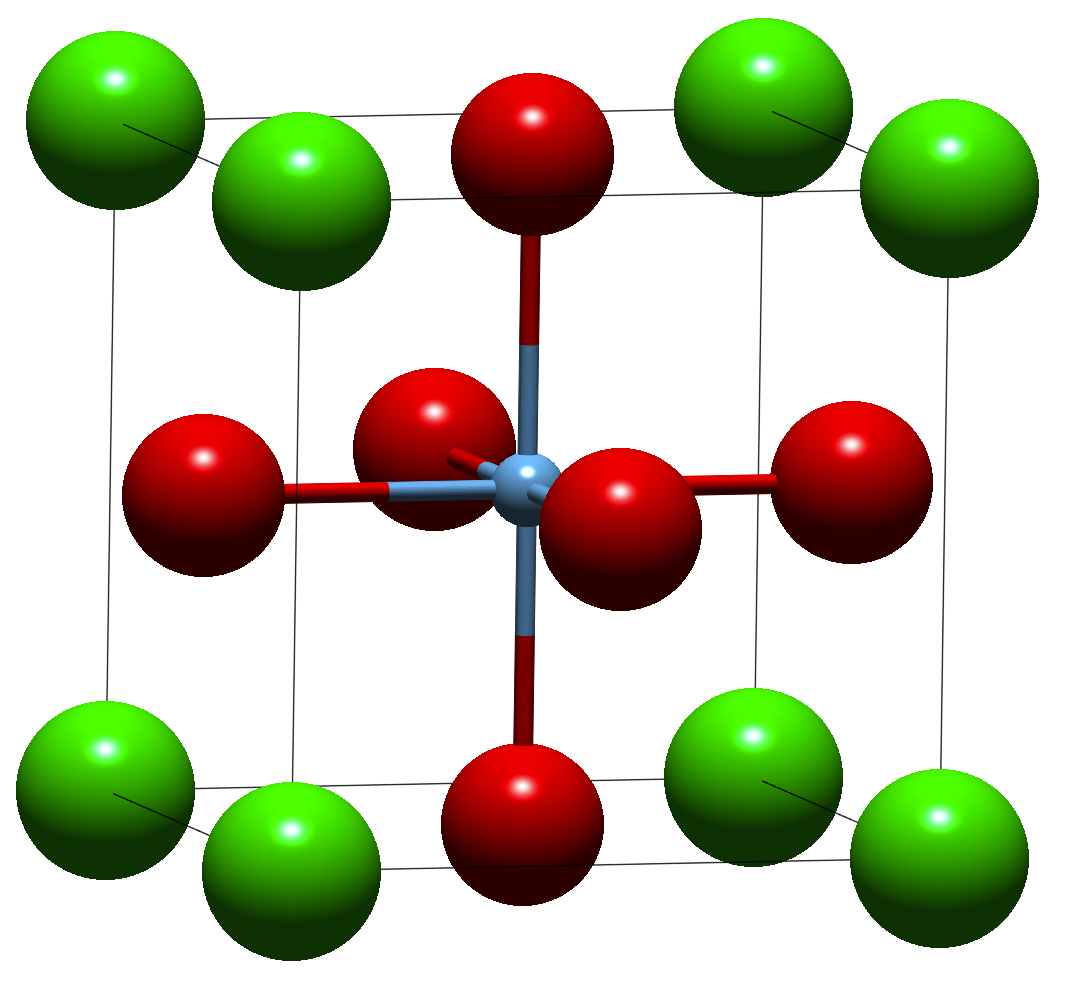
\includegraphics[width=\marginparwidth]{stocell.png}
%}{-5}

Strontium titanate, \ce{SrTiO3}, is a cubic perovskite at room temperature. It has a lattice parameter 3.905 \si{\angstrom}. The unit cell of \ce{SrTiO3} is depicted in \figureref{stocell}. At room temperature, \ce{SrTiO3} takes the form of the prototype cubic perovskite described in \sectionref{subsec:background.perovskites}, with Sr atoms on the primitive lattice sites, Ti atoms at the body center, and O atoms on the face centers of the cubic cell. The band gap of strontium titanate is 3.2~eV,\cite{Cardona:1965vw} corresponding to the ultraviolet range of the electromagnetic spectrum. In this work, \ce{SrTiO3} was selected as a material for \ce{Fe2O3} film growth on single crystal substrates. 
 
Depending on orientation, ideal \ce{SrTiO3} surfaces can be polar or nonpolar. The (001) face of strontium titanate is nonpolar, existing as neutral planes of either SrO or \ce{TiO2}. The (110) and (111) surface are polar. In the case of (110) oriented planes, possible surface terminations are \ce{SrTiO^{4+}} and \ce{O2^{4-}}. For (111) oriented surface, surface terminations are \ce{SrO3^{4-}} and \ce{Ti^{4+}}. Projections of the (001), (110), and (111) surfaces are shown in \figureref{stoterms}. The effect of substrate surface polarity on photochemical behavior of supported films is discussed later in this document.

\begin{figure}
%	\begin{whole}
	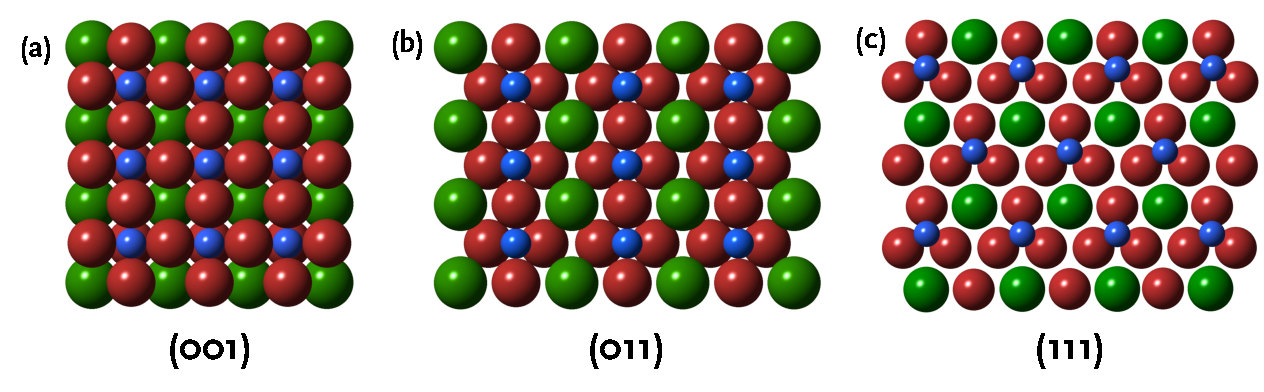
\includegraphics[width=\textwidth]{stoterms.pdf}
		\caption[Low-index \ce{SrTiO3} surface terminations]{%
			Models of the \ce{SrTiO3} (001), (011), and (111) surface. 
			Red, green, and blue represent oxygen, strontium, and oxygen 
			atoms respectively. The (001) surface is terminated by neutral 
			\ce{TiO2} and \ce{SrO} terminations. The (011) and (111) 
			terminations are polar. The (011) surface is either \ce{SrTiO} 
			or \ce{O2} terminated and the (111) surface is terminated by 
			either Ti or \ce{SrO3} layers.}
	\label{fig:stoterms}
%	\end{whole}
\end{figure}

%\subsubsection{Barium Titanate}
%\label{subsubsec:background.bto}
%
%\sidefigure[AFM micrograph of a \ce{BaTiO3} surface]{%
%	AFM micrograph of a \ce{BaTiO3} surface showing 180\si{\degree} 
%	and 90\si{\degree} domain boundaries.
%	\label{fig:btosurface}
%	}{%
%	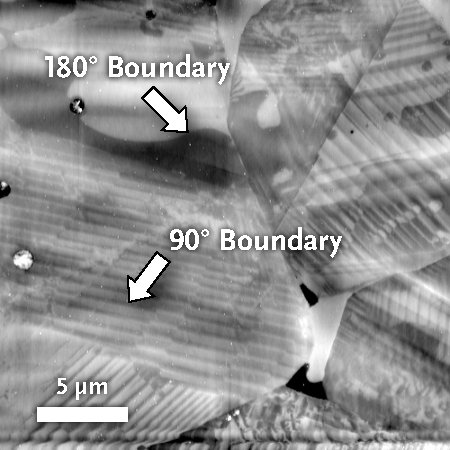
\includegraphics[width=\marginparwidth]{btosurface.pdf}
%}{-1}
%
%\ce{BaTiO3} is a tetragonally distorted perovskite with a band gap of 3.2~eV. \ce{BaTiO3} is typically an n-type semiconductor, owing to presence of oxygen vacancies. When cooled below its Curie temperature of 120 \si{\degreeCelsius}, the unit cell shifts from cubic to tetragonal symmetry, slightly elongating along the [001] direction. The tetragonal unit cell has lattice parameters of a = 3.98 \si{\angstrom} and c = 4.03 \si{\angstrom} at room temperature.\cite{ForsberghJr:1949vl,Heywang:1971uv} This transition is paraelectric-to-ferroelectric, giving rise to ferroelectric polarization along the c-axis. The spontaneous polarization Ps at room temperature is 26 \si{\micro\coulomb\per\cm\squared}, and exists along the elongated [001] direction. This phase transition and resultant unit cell is shown in \figureref{btocell}. The figure shows how the ferroelectric polarization arises from the distortion of the Ti--O octahedra. 
%
%\begin{figure}
%	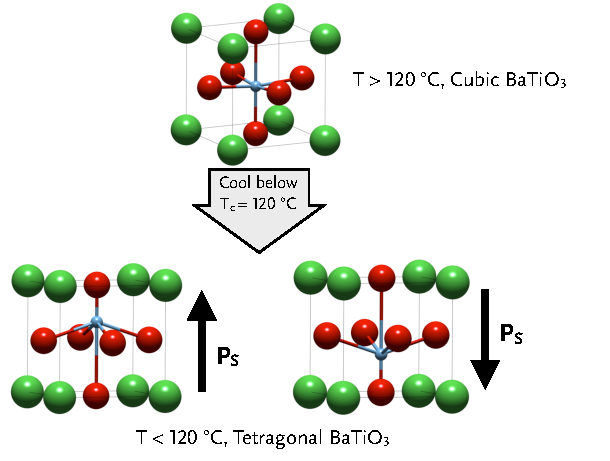
\includegraphics[width=\textwidth]{btocell.pdf}
%	\caption[\ce{BaTiO3} ferroelectric phase transition]{%
%		The cubic \ce{BaTiO3} unit cell transitioning to the 
%		ferroelectric tetragonal phase. The distortion of the 
%		Ti--O octahedra is exaggerated in this diagram.}
%	\label{fig:btocell}
%\end{figure}
%
%In this work, \ce{BaTiO3} is used as a polycrystalline substrate for \ce{Fe2O3} film growth. As discussed earlier in the section on ferroelectricity, bulk specimens of \ce{BaTiO3} contain numerous ferroelectric domains. The elongated [001] direction of the unit cell is defined to be the direction of positive ferroelectric polarization. This crystal direction can exist in the $\pm$x, $\pm$y, or $\pm$z direction.\cite{ForsberghJr:1949vl} This constraint on the direction of ferroelectric polarization gives rise to two types of domain boundaries, 90\si{\degree} and 180\si{\degree} boundaries.\cite{Anonymous:7uC1r_sG} The angle refers to the change in direction of polarization when crossing the boundary. 90\si{\degree} boundaries are confined to (110) planes and intersect the surface at straight lines. 180\si{\degree} planes are not confined to a single crystal habit, and so appear as curved lines. \figureref{btosurface} shows an AFM micrograph of a polished \ce{BaTiO3} surface, with 90\si{\degree} and 180\si{\degree} domains identified. The domains of \ce{BaTiO3} have a strong effect on the photochemical activity of \ce{TiO2} films supported on \ce{BaTiO3} substrates. The effect of these domains on the photochemical activity of \ce{Fe2O3} is reported in this document. 


\subsubsection{Bismuth Ferrite}
\label{subsubsec:background.bfo}

\begin{figure}
\begin{center}
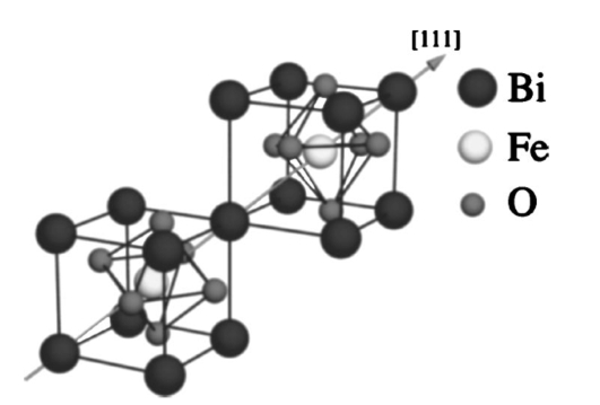
\includegraphics[width=0.6\textwidth]{bfocell.pdf}
\caption[Pseudo-cubic \ce{BiFeO3} unit cell]{%
	Pseudo-cubic \ce{BiFeO3} unit cell, showing rhombohedral [111] 
	distortion and resulting ferroelectric polarization.\cite{Catalan:2009ca}}
\label{fig:bfocell}
\end{center}
\end{figure}
%\sidefigure[Pseudo-cubic \ce{BiFeO3} unit cell]{%
%	Pseudo-cubic \ce{BiFeO3} unit cell, showing rhombohedral [111] 
%	distortion and resulting ferroelectric polarization.\cite{Catalan:2009ca}
%	\label{fig:bfocell}
%	}{%
%	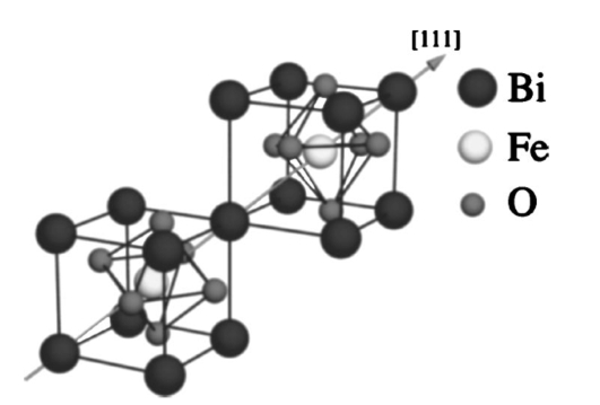
\includegraphics[width=\marginparwidth]{bfocell.pdf}
%}{-11}

Bismuth ferrite, \ce{BiFeO3}, is ferroelectric, rhombohedrally distorted perovskite with a Curie temperature of \texttildelow830-850 \si{\degreeCelsius}.\cite{Kornev:2007jr,Catalan:2009ca,Anonymous:htMDB4Eh,Miao:2008fz} The perovskite unit cell has the lattice constants $\text{a}_{\text{Rh}}$~=~3.965~\si{\angstrom} and $\text{\textalpha}_{\text{Rh}}$~=~89.4\si{\degree}.\cite{Kubel:1990kd} Because the rhombohedral distortion is so small ($\text{\textalpha}_{\text{Rh}}$~=~89.4\si{\degree} versus 90\si{\degree} for a cubic cell), crystal directions and planes are typically referenced using the pseudocubic perovskite cell rather than the more complex rhombohedral or hexagonal systems.  The pseudocubic unit cell is depicted in \figureref{bfocell}. Bulk \ce{BiFeO3} is a p-type oxide semiconductor with reported band gaps of 2.3~eV to 2.8~eV.\cite{Ihlefeld:2008hl,Clark:2007bt,Kumar:2008fr} The p-type conductivity arises from the loss of volatile bismuth during synthesis, resulting in cationic vacancies in the crystal lattice. 

The ferroelectric polarization vector is observed along the pseudocubic <111> family of directions.\cite{Catalan:2009ca} This gives rise to three possible types of domain walls: 180\si{\degree}, 109\si{\degree}, and 71\si{\degree}. 180\si{\degree} walls separate domains with antiparallel polarization vectors, for example, [111] and [\={1}\={1}\={1}]. If two of the components of the polarization vector are reversed across the boundary, it is a 109\si{\degree} wall, and if only one component is reversed, the boundary is a 71\si{\degree} wall. Equilibrium domain walls are constrained to certain orientations. 71\si{\degree} walls exist parallel to {110} planes, 109\si{\degree} walls parallel to \{100\} planes, and 180\si{\degree} walls on any plane containing the polarization vectors separated by the boundary.\cite{Streiffer:1998vt}

In contrast to \ce{BaTiO3}, for which spatially selective reactivity has been observed and characterized, \ce{BiFeO3} has a band gap in the visible spectrum, is a p-type semiconductor, and has <111> type ferroelectricity. The spatially-selective photochemical properties of \ce{BiFeO3}, taking into account these differences, were studied and are reported in this document.

